\documentclass[pdftex,12pt,a4paper]{article}
\usepackage[utf8]{inputenc}
\usepackage[english,brazil]{babel}
\usepackage[T1]{fontenc}
\usepackage[top=3cm,left=3cm,right=2cm,bottom=2.5cm]{geometry}
\usepackage{indentfirst}
\usepackage[pdftex]{graphicx}
\usepackage[table]{xcolor}
\usepackage{makeidx}
\usepackage{colortbl}
\usepackage{longtable}
\usepackage{multirow}
%\usepackage{natbib}
\usepackage[alf]{abntcite}
\usepackage{float}
\usepackage{tabularx}
\usepackage{setspace}
\usepackage{appendix}
\usepackage{tocloft}

\makeatletter
\renewcommand{\@dotsep}{\cftnodots}
\makeatother

%\singlespacing
\onehalfspacing
%\doublespacing
\pagestyle{myheadings}
%\bibpunct{(}{)}{;}{a}{,}{,}
\graphicspath{{images/}}
\setlength{\parindent}{2cm}

\def\citacao#1#2{\list{}{\rightmargin#2\leftmargin#1}\item[]}
    \let\endcitacao=\endlist

\usepackage{estilos_custom}

\title{Desenvolvimento de jogos utilizando as tencnologias dos navegadores compat�veis com HTML5}
\author{Willian Araujo Molinari}
\begin{document}
\newcommand{\cabecalhotabela}
{
Afirmativas &
\scriptsize{Se aplica totalmente � empresa} &
\scriptsize{Se aplica muito � empresa} &
\scriptsize{Se aplica parcialmente � empresa} &
\scriptsize{N�o se aplica � empresa} &
\scriptsize{N�o sabe} \\
}


\newcounter{titem}
\newcommand{\tabitem}{\stepcounter{titem}\arabic{titem} {--} }
\newcounter{citem}[titem]
\newcommand{\cellitem}{\stepcounter{citem}\alph{citem}. }
\newcommand{\fimcel}{ & & & & & \\}

\newcounter{thead}
\newcommand{\tablehead}[2]{\cellcolor[gray]{0.6}\stepcounter{thead}\arabic{thead} {--} #1 #2}
\newcounter{cellitem}[thead]
\newcommand{\tcitem}{\stepcounter{cellitem}\arabic{thead}.\arabic{cellitem}. }

\newcommand{\subheader}{Objetivo & Fundamenta��o Te�rica \\ }

\newcommand{\iso}{NBR ISO/IEC 17799:2001}
\newcommand{\isop}{(NBR ISO/IEC 17799:2001)}

%%% Macros das tabelas de dados
\newcommand{\theadone}{Quest�o & Item & 0 & 1 & 2 & 3 & 4 \\}
\newcommand{\CA}{Controle de Acesso}
\newcommand{\CI}{Classifica��o~e Controle dos Ativos~de~Informa��o}
\newcommand{\CO}{Conformidade}
\newcommand{\DS}{Desenvolvimento e Manuten��o de Sistemas}
\newcommand{\GC}{Gest�o de Contratos}
\newcommand{\GN}{Gest�o da Continuidade do Neg�cio}
\newcommand{\GO}{Gerenciamento das Opera��es e Comunica��o}
\newcommand{\PS}{Pol�tica de Seguran�a}
\newcommand{\SO}{Seguran�a Organizacional}
\newcommand{\SF}{Seguran�a F�sica e de Ambiente}
\newcommand{\SI}{Seguran�a da Informa��o }
\newcommand{\SP}{Seguran�a em Pessoas}
\newlength{\tlen}
\setlength{\tlen}{6cm}



  %%% Capa
  \thispagestyle{empty}
\begin{center}
\large Faculdade de Tecnologia de S�o Paulo - FATEC-SP \\
\large Departamento de Automa��o de Escrit�rios e Secretariado \\
\large Curso de Automa��o de Escrit�rios e Secretariado \\
\vspace{8cm}
\huge Seguran�a da Informa��o \\ \Large Um estudo sobre a aplica��o da seguran�a
e gest�o de contratos \\
\vspace{9cm}
\large Fernanda Rodrigues Arraiol
\end{center}

  \clearpage

  %%% Folha Rosto
  \thispagestyle{empty}

\vspace{3cm}
\begin{center}
WILLIAN ARAUJO MOLINARI \\
\vspace{3cm}
\huge Desenvolvimento de jogos casuais utilizando as tecnologias dos navegadores compatíveis com HTML5 \\
\vspace{0.5cm}
\large.\\
\hspace{6cm} \begin{minipage}{0.5\textwidth}
Trabalho de Conclusão de Curso apresentado como exigência parcial para
obtenção do grau de bacharel em Sistemas de Informação, à Faculdade
FAFIL do Centro Universitário Fundação Santo André. \\
\\
Relatório final apresentado ao Programa de Incentivo à Iniciação
Científica do Centro Universitário Fundação Santo André.\\
\\
Orientador: \\
Prof. Tomaz Mikio Sasaki
\end{minipage}
\vspace{2cm}

\huge Santo André \\ 2011
\end{center}

  \clearpage

  %%% Agradecimentos
  \thispagestyle{empty}
\begin{center}
%%% teste
\end{center}

\begin{flushright}\footnotesize
\vspace{17cm}

\textbf{Agradecimentos} \\

Escrever agradecimentos aqui
\end{flushright}

  \clearpage

  %%% Ep�grafe
  \thispagestyle{empty}
\begin{center}
%
\end{center}
\vspace{21cm}

\begin{flushright}
``\emph{Os importantes problemas que enfrentamos não podem ser resolvidos com o
mesmo raciocínio de quando os criamos}''.  \\ (Albert Einstein)
\end{flushright}

  \clearpage

  %%% �ndice
  \renewcommand\thepage{}
  \setcounter{tocdepth}{1}
  \tableofcontents
  \clearpage


  %%% Lista de Figuras
  \listoffigures
  \clearpage

  %%% Lista de Tabelas
  \listoftables
  \clearpage

  %%% Cap�tulos
  \begin{abstract}

Este trabalho tem como objetivo apresentar por meio de um estudo
baseado no atual estado do HTML5 e dos navegadores, a viabilidade de
se desenvolver jogos casuais que possam ser executados diretamente
nos navegadores dos dispositivos compatíveis com essa tecnologia.
Para provar a viabilização da tecnologia este trabalho faz comparações
com as principais ferramentas utilizadas atualmente, assim mostrando
as principais vantagens e desvantagens em diversos aspectos relevantes
na área de desenvolvimento de jogos casuais.

\vspace{5cm}

\textbf{Palavras-Chave: HTML5, jogos casuais}
\end{abstract}

  \thispagestyle{empty}{\selectlanguage{english}
\begin{abstract}

\noindent With the HTML5 technologies is possible to create great casual games
that run on the internet without third part products. This paper has as its main objective, to show the feasibility to develop
casual games that run on HTML5 compatible browsers based on the
actual HTML5 state. To show the technology feasibility this paper will
compare the main advantages and disadvantages on various casual game
development area relevant aspects.

\vspace{5cm}
\textbf{Keywords: HTML5, casual games}
\end{abstract}
}

  \renewcommand\thepage{\arabic{page}}
  \setcounter{page}{1}
  \section{Introdução}

A web tem crescido muito nos últimos anos, e suas novas ferramentas trazem várias
facilidades para desenvolver aplicações para a web, e isso também pode ser aplicado
a jogos casuais, trazendo também para os games uma facilidade de distribuição e portabilidade,
por utilizar apenas um browser moderno.

Mostrar as possibilidades de inovação e negócio que as novas tecnologias implementadas
nos navegadores compatíveis com HTML5 trazem para o mundo de desenvolvimento de jogos casuais,
comparando-as com as tecnologias existentes no mercado.

O objetive desse trabalho é apresentar os conceitos e utilizações das novas ferramentas utilizadas
nos navegadores compatíveis com HTML5, focando principalmente em HTML5 e Javascript.
Será abordado a história do HTML, mostrando sua evolução com o passar do tempo, chegando
a seu estado atual, explorando quais a sua finalidade e quais os problemas que ele foi criado para resolver.
Logo em seguida será abordado a história do Javascript e sua evolução até seu estado
atual, mostrando qual a sua ligação com o HTML e como a sua evolução é importante
para o futuro da web, não somente com páginas comuns, mas com experimentos multimídia também.

Será apresentada também uma introdução do CSS e seu uso, para assim formar "o ciclo
do HTML5", que é formado por HTML, Javascript e CSS.

Com uma visão maior de HTML5, o trabalho vai focar em seus recursos e como isso pode
ser usado para o desenvolvimento de games. A ideia é descrever cada um de seus recursos
chave e mostrar passo a passo, com exemplos, onde ele pode ser aplicado e porque isso
é viável e útil, comparando com as tecnologias existentes no mercado atualmente. Para
a comparação serão avaliados alguns itens como, performance, dependências, portabilidade, recursos e viabilidade.

Com o grande crescimento da tecnologia dos navegadores, muita coisa se tornou possível
e viável, uma delas é o desenvolvimento de jogos casuais. Com a constante evolução
dos interpretadores de Javascript, HTML e CSS dos navegadores mais populares, é possível
desenvolver jogos simples e divertidos e conseguir um bom retorno com isso. Atualmente,
várias tecnologias são utilizadas para se fazer jogos para a web, cada uma com suas
vantagens e limitações, e o HTML5 (e seus complementos), entrou na competição, prometendo
se tornar o padrão para multimídia na web.

Javascript é uma linguagem de programação com capacidades de Orientação a objetos comumente utilizada em
navegadores \cite{flanagan2006javascript}, sendo que, nesse contexto ela tem seu propósito extendido com objetos que permitem
aos scripts uma interação com o usuário, controlando o navegador e alterando o conteúdo
do documento que aparece na janela do navegador.
Utilizando a interação com o navegador que o Javascript proporciona, é possível movimentar
objetos pelo navegador, adicionar conteúdo, criar novos objetos, fazer desenhos, guardar
informações, entre outras coisas, bastando manipular o HTML da página.

HTML é uma linguagem de marcação de hipertexto que é utilizado como base para a internet
atual. O HTML mudou bastante desde sua versão inicial em 1991
\cite{powell2003html}, no início o HTML não era muito definido, e não tinha um padrão, até que que a
IETF (Internet Engeenering Task Force) começou a padronizá-lo em 1995, lançando a
primeira versão padronizada do HTML, que ficou conhecida como HTML 2.0.
Com o tempo o HTML foi se tornando mais padronizado, ganhando validações e novas integrações
(com CSS por exemplo), tornando-o mais versátil e adequado as novas necessidades da
web. Outra vantagem que a padronização trouxe, foi a facilidade de implementação pelos
navegadores, que agora implementavam com menos frequência o seu próprio estilo de marcação.
A ultima versão do HTML desenvolvida é o HTML5, que traz funcionalidades que dão um
olhar diferente para a internet, ou seja, ao invés de apenas se preocupar com texto
e formatação, o HTML5 visa atender as necessidades multimídia da internet, cobrindo
todos os espaços multimídia que tiveram que ser contornados com outras tecnologias,
como por exemplo vídeo, audio e desenho.
Com o crescimento do HTML, algumas coisas foram alteradas na parte de visualização,
removendo algumas tags que eram utilizadas para isso, como a tag font por exemplo.
Com a remoção dessas tags surgia a utilização de outra forma para
estilização de páginas, o CSS.

CSS é uma linguagem para criação de folhas de estilo, que interage com um documento
HTML, dando a ele uma melhor visualização, manipulando fontes, cores e espaçamentos.
A versão 2 do CSS se tornou padrão em maio de 1998, \cite{zeldman2009designing},
e atualmente está sendo desenvolvida a versão 3, que já está parcialmente implementada
nos navegadores compatíveis com HTML5, apesar de ainda estar em construção (assim como o HTML5).
Utilizando essas tecnologias emergentes da web é possível fazer jogos casuais simples
e divertidos. Uma das definições que ajuda a resumir um jogo casual é: "Um jogo casual não exige do jogador horas de
dedicação para cada seção de jogo, o jogo deve ser jogado aos poucos, em pequenas
porções, isso vai ajudar o jogo a se adequar a quantidade de tempo que os jogadores
de jogos casuais podem dedicar a ele. \cite{trefry2010casual}.
A tecnologia que domina o mercado de jogos casuais atualmente é o flash, que devido
a sua grande adoção na época que a internet carecia de multimídia, se tornou "padrão"
em todos os computadores atuais, apesar de ser um software de terceiros instalado
como plugin para os navegadores. Java tem uma pequena porcentagem no total de jogos
na web, e é pouco usada ultimamente, diferentemente do framework Unity, que pode exportar
os games para a web, e tem crescido bastante desde seu lançamento.

O HTML5 traz a possibilidade de suprir várias funcionalidades de cada uma dessas tecnologias,
com a vantagem de ser um padrão implementado pelos empresas que desenvolvem os navegadores
mais conhecidos do mercado, e que já estão fazendo seus browsers para celulares e
video games, abrindo mais possibilidades para um jogo simples estar disponível em mais plataformas.

  \section{Javascript, HTML5 e a evolução dos navegadores}

%TODO: Fazer um resumo da arquitetura da internet

Os navegadores evoluíram muito nos últimos anos e com essa evolução
veio a possibilidade de utilização de tecnologias que integram
diretamente com o navegador, provendo muitas possibilidades de uso com
a vantagem de terceirizar o trabalho da implementação multi-plataforma
de uma aplicação, pois as empresas que desenvolvem os navegadores
terão todo esse trabalho pelo desenvolvedor. Essa se tornou uma das
grandes vantagens do HTML5, e com sua evolução constante, é possível
construir diretamente no navegador muitas coisas que atualmente necessitam
de ferramentas de terceiros, apenas utilizando javascript para a
manipulação.

\subsection{HTML e sua evolução}

HTML é uma linguagem de marcação de hipertexto que é utilizada como base para a internet
atual. O HTML mudou bastante desde sua versão inicial em 1991. \cite{powell2003html}.
No início o HTML não era muito definido, e cada
navegador definia novas tags que tinham funções diferentes,
não seguindo um padrão específico, o que dificultava
bastante o trabalho dos desenvolvedores da época.
O tempo se foi se passando e após algum tempo um esforço de padronização da linguagem
começou a ser organizado e, em 1995 o IETF começou o processo de
padronização, lançando a primeira versão padronizada do HTML, que ficou conhecida como HTML 2.0.
Com o tempo o HTML foi se tornando mais padronizado, ganhando validações e novas integrações
(com CSS por exemplo), tornando-o mais versátil e adequado às novas necessidades da
internet.
Essa padronização resolveu vários problemas de fragmentação, onde cada
navegador implementava sua funcionalidade específica, pois os agora
eles poderiam começar a seguir as especificações padronizadas,
facilitando as implementações de cada navegador, que agora implementavam com
menos frequência o seu próprio estilo de marcação.
As primeiras página HTML eram feitas apenas com HTML, ou seja, era
responsabilidade do HTML cuidar de toda a diagramação do site para que
ele fosse agradável para o visitante, e muitos tipos de
desenvolvimento foram adotados, utilizando os melhores elementos para
conseguir diagramar uma página sem se importar com a semântica do
documento. Com a chegada do site de busca da Google as coisas mudaram bastante, pois
agora não havia apenas humanos olhando para a página, robôs também
estavam passando por ali e precisavam entender da melhor maneira
possível aquele conteúdo para poder adicionar a página no lugar certo
nos índices de busca. Com isso o HTML começa a ser utilizado de uma
forma mais estruturada, utilizando o CSS para estilizar a visualização,
assim, removendo do HTML a responsabilidade de lidar com cores, tipos de
fonte e etc. Com as responsabilidades bem divididas, o CSS pode tratar
do que é mostrado para o usuário e o HTML cuidar do que é mostrado
para os robôs, mantendo o melhor dos dois pontos.

%TODO: falar de XHTML

A ultima versão do HTML que está em desenvolvimento é o HTML5, que
traz novos marcadores para definir melhor a semântica dos documentos e
traz também funcionalidades que dão um olhar diferente para a internet,
ou seja, ao invés de apenas se preocupar com texto e formatação, o HTML5
visa atender às necessidades multimídia da internet, cobrindo todos os
espaços multimídia que tiveram que ser contornados com outras tecnologias,
como por exemplo vídeo, áudio e desenho.

Ainda é difícil dizer o que é parte do HTML5, pois atualmente o HTML5
é apenas um rótulo utilizado para identificar um conjunto de recursos
obtidos através do navegador, entre esses recursos está a nova
linguagem de marcação, que possui diversas novas funcionalidades para
deixar um documento mais semântico.
Alguns exemplos das novas funcionalidades que compõe esse novo ambiente:

\begin{itemize}
  \item Nova tag <article> para delimitar artigos;
  \item Nova tag <section> para delimitar seções;
  \item Nova tag <aside> para delimitar menu lateral;
  \item Nova tag <audio> para inserir áudio na pagina;
  \item Nova tag <video> para inserir vídeo na pagina;
  \item Novos tipos para a tag <input> para inserir mais facilmente:
  data, url, numero, dia, mês, ano, horário, email e outros;
  \item History API, para poder ter acesso ao histórico de visitas do
  usuário, pedindo-lhe permissão para esse acesso;
  \item GeoLocation: Utilizado para saber onde o usuário está localizado no
  mundo;
  \item WebWorkers: Utilizado para executar scripts independentemente das ações
  da página;
  \item WebSockets: Utilizado para criar uma conexão persistente entre
  o servidor e o navegador;
  \item LocalStorage: Utilizado para guardar informações no navegador
  do usuário;
  \item Offline cache: Utilizado para salvar os arquivos necessários
  para que a aplicação fique disponível quando o usuário não estiver
  conectado à internet;
  \item Canvas: Para fazer desenhos e importar imagens de uma maneira
  mais fácil, e rápida, não dependendo da separação de objetos do DOM;
  \item SVG: Para criação e manipulação de vetores diretamente no
  navegador;
\end{itemize}

\subsection{Javascript e sua evolução}

Javascript é uma linguagem que foi criada em 1995 por Brendan Eich,
um engenheiro da Netscape, e foi lançada no começo de 1996 com o
Netscape 2 \cite{mdnjavascript}, sendo padronizada pela Ecma
Internacional em 1997, lançando assim a primeira versão do ECMAScript.
Javascript é uma linguagem de programação com capacidades de orientação a objetos e que tem como uma das suas principais
utilizações a manipulação de objetos em navegadores \cite{flanagan2006javascript}, sendo que, nesse contexto,
ela tem seu propósito estendido com objetos que permitem aos scripts uma interação com o usuário,
controlando o navegador e alterando o conteúdo do documento que aparece na janela do navegador.
Desde sua padronização, o Javascript vem sendo alterado e
recebeu algumas atualizações, sendo que a versão comumente
utilizada (e considerada estável) é a versão 3, padronizada em 1999.
O Javascript é muito utilizado nas paginas de internet atuais para
diversas finalidades, seja validação de simples formulários até
animações mais complexas. Várias bibliotecas foram desenvolvidas para
dar um poder maior ao desenvolvedor, sendo uma das mais conhecidas o
jQuery, que ajuda o desenvolvedor a ser mais produtivo, facilitando a
pesquisa por objetos dentro do DOM, facilitando a criação de efeitos
básicos, dando uma interface simples para alterar CSS e outras coisas.

\subsection{CSS e sua evolução}

CSS é uma linguagem para criação de folhas de estilo, que foi criada
para facilitar a criação de páginas para internet, comparada as técnicas da época de
1990, o CSS fornece um controle bem maior sobre as páginas. \cite{schmitt2009css}.
O CSS interage com um documento HTML, dando a ele uma melhor visualização, manipulando
fontes, cores e espaçamentos, assim deixando a diagramação e visualização do documento
separado da estrutura do mesmo, deixando para o HTML apenas a
responsabilidade de manter um documento estruturado e semântico.
A versão mais utilizada atualmente, e considerada estável para utilização, é a versão 2
que se tornou padrão em maio de 1998. \cite{zeldman2009designing}.
A versão 3 está em desenvolvimento e alguns dos navegadores atuais mais populares
já suportam muitas de suas funcionalidades, e estão constantemente
adicionando as novas funcionalidades assim que são lançadas.
Com CSS3 é possível fazer muitas coisas que demandavam muito trabalho
do desenvolvedor com CSS2. Um exemplo bem simples do quanto o CSS3
pode ajudar na criação de um layout são os botões com cantos
arredondados, que era muito trabalhoso de se fazer utilizando CSS2 e
dependia de várias imagens juntas para fazer cada um dos cantos e
bordas do botão. O CSS3 possui essa funcionalidade implementada, e os
botões podem ter cantos arredondados facilmente utilizando a
propriedade \textit{border-radius}, tirando toda essa complexidade das mãos do
desenvolvedor.

\subsection{A evolução dos navegadores}

Os navegadores nasceram muito antes da interface gráfica,
e é possível notar sua constante evolução para suprir as necessidades
dos usuários e desenvolvedores \cite{robbins2006web}. No início, os
navegadores eram apenas texto preto sobre um fundo cinza, e foi assim
nos primórdios da internet, enquanto o Mosaic e o Lynx eram os
navegadores modo texto famosos, sendo que o Mosaic foi o primeiro
navegador a mostrar as imagens junto com o texto.
Em 1994 foi lançado o Netscape 0.9, que
trouxe várias inovações para a internet, e dois anos depois a
Microsoft contra ataca com o Internet Explorer 3.0, com várias
funcionalidades novas, inclusive o suporte a folhas de estilo (e
introduzindo o CSS), e iniciando o que chamam de "A guerra dos
navegadores". Essa guerra foi travada entre a Microsoft e a Netscape
por muitos anos e trouxe muitas coisas boas e ruins para a internet. O
impacto positivo foi a aceleração do desenvolvimento para essas
plataforma, e o impacto negativo foi a grande falta de padrão para os
desenvolvedores, pois cada navegador implementava HTML utilizando seu
próprio formato. A Microsoft conseguiu uma grande vantagem quando lançou
o Windows 95 OSR2 que já tinha o internet explorer gratuitamente
\cite{asleson2006foundations}, e venceu oficialmente a guerra dos navegadores quando a
Netscape foi comprada pela AOL(America Online). A Netscape deixou o código-fonte
de seu navegador liberado para quem quisesse continuar o projeto,
e a Mozilla utilizou esse código para começar o desenvolvimento
do que futuramente seria o Firefox.
Em 2005 foi lançada a primeira versão do Firefox e a Microsoft começa
a perder seu reinado absoluto com navegadores. O Firefox conseguiu uma
boa fatia do mercado de navegadores, e a Microsoft ficou para trás em
termos de tecnologia e segurança a partir da versão 6 do Internet Explorer.

Com o passar dos anos, outros navegadores entram nessa disputa, entre
eles estão o Opera, que tem uma pequena parte do mercado mas está em
constante desenvolvimento, e o Chrome da Google, que está entre os
mais rápidos e seguros navegadores da atualidade.
Novamente uma Guerra dos navegadores começa, mas dessa vez um pouco
mais controlada, pois existe um órgão regulamentador da internet que
todos os navegadores procuram seguir e se adequar, ele se chama W3C,
e seu papel nessa história é dizer o que
é padrão e o que não é, assim fazendo que a interface para os
desenvolvedores seja o mais parecida possível entre todos os
navegadores.
Ainda hoje cada navegador possui um conjunto diferente de funcionalidades
do HTML5 ou CSS3, o que faz com que nem todos os recursos funcionem em todos
os browsers, e sua própria implementação do
interpretador de Javascript, o que faz alguns serem mais rápidos que
outros. E uma das grandes vantagens atuais, principalmente falando de
aplicações ricas, que tem um uso intenso de Javascript, é a velocidade
desse interpretador e o suporte às novas funcionalidades que o HTML5
propõe.
Os principais navegadores da atualidade são: Opera, Firefox, Internet
Explorer e Chrome. Todos estão implementando, cada um em seu ritmo, as
funcionalidades do HTML5, e estes, em suas ultimas versões, serão usados
como base para os estudos desse trabalho.

  \section{Jogos casuais e sua evolução}

Nesse capítulo será abordado o que são os jogos casuais, como eles
evoluíram com o passar dos tempos, qual o estado desse tipo de jogo
desenvolvido para internet e a influencia deles no ritmo de vida das
pessoas.

\subsection{Os jogos casuais}

É possível definir jogos casuais como aquele jogo que pode ser jogados em um curto período
de tempo. Conforme \citeonline{trefry2010casual}, são jogos rápidos e acessíveis.
Diferentemente dos grandes jogos criados por grandes e conceituadas
empresas do mundo dos jogos, os jogos casuais não precisam de grandes
equipes para serem desenvolvidos, uma equipe pequena de 3 ou 4 pessoas
pode fazer um jogo simples e divertido, e em alguns casos apenas um
desenvolvedor pode criar um jogo casual se possuir habilidades em
diferentes áreas (como design e programação).

Uma vantagem dos jogos casuais é a facilidade em divulgá-lo. De acordo com
\citeonline{ozcan2010recent}:

\begin{singlespacing}
\begin{citacao}{4cm}{0cm}\footnotesize \emph
    ``O tempo de entrada para os jogos casuais em navegadores é pequeno,
    pois eles são fáceis de se recomendar para os amigos. Pessoas jogando
    algum jogo de navegador são uma ótima maneira de atrair mais
    pessoas para jogar um determinado jogo.''
\end{citacao}
\end{singlespacing}

Atualmente, os jogos casuais possuem muitas vantagens, pois a conexão
com os amigos é feita muito facilmente, portanto, os jogadores
recomendam uns para os outros o jogo que está jogando. Um dos motivos
que facilita essa proliferação é a portabilidade, pois o jogo pode
estar em um dispositivo móvel, ou em um computador qualquer, acessível
via internet, e etc.

\cite{ozcan2010recent} já comentava sobre a facilidade que a
portabilidade desse tipo de jogo trazia para a vida das pessoas, e
consequentemente para o desenvolvedor. Segundo ele a portabilidade é um
dos grandes motivos do sucesso desses jogos, pois a possibilidade de
jogar em qualquer lugar, em curtos períodos no meio da vida cotidiana
do jogador, faz total diferença para quem não é um jogador nato.

Tendo isso em mente, é possível imaginar, um jogo divertido e desafiador
sendo passado entre amigos, utilizando diversos meios, preenchendo os
tempos vagos de cada um, trazendo pequenos desafios divertidos que
trazem ao jogador a vontade de compartilhar e passar esse desafio para
o amigo utilizando o jogo, o que faz ele ser cada vez mais popular e
divertido.

\subsection{A evolução dos jogos casuais no navegador}

Podemos dizer que os jogos casuais para computador começaram com
o paciência criado para o Windows pela Microsoft em 1990 \cite{trefry2010casual}.
Nessa época o mouse estava começando a ser introduzido no mercado e
eles precisavam de algo que fizesse as pessoas entenderem como o mouse
funcionava e quais suas utilidades. O paciência fez um ótimo trabalho
nessa área e inclusive hoje ele pode se considerar o jogo mais jogado
do mundo conforme \citeonline{trefry2010casual}.

Conforme \citeonline{trefry2010casual}, o termo "jogo casual" tem se
modificado bastante ao longo do tempo, e está sendo utilizado para
diversos tipos de jogos. Algumas características comuns entre os jogos
que são considerados casuais são:

\begin{itemize}
    \item Regras e objetivos devem ser claros;
    \item Os jogadores devem conseguir pro-eficiência rapidamente;
    \item O jogo se adapta a vida e a agenda do jogador;
    \item O conceito do jogo utiliza conteúdos familiares e coisas da vida.
\end{itemize}

Várias grandes empresas tem investido em jogos casuais, um grande
exemplo é a Nintendo com o Nintendo Wii, que grande parte dos jogos
são casuais, simples de aprender a jogar e divertidos para se jogar
em um curto período de tempo.
A Microsoft tem feito o mesmo com o Kinect, que
possui como jogo principal (o jogo que apresentou a plataforma), um
conjunto de jogos casuais que são simples e divertidos para se jogar
em grupos.

Quando os jogos começaram a ser desenvolvidos para executar
diretamente no navegador, era fácil de ver que a grande maioria deles
se enquadravam na descrição de jogos casuais que é usada nesse
trabalho, e ainda hoje, a grande maioria desses jogos ainda seguem
esse mesmo padrão, e há uma explicação simples para esse
acontecimento: Quando um desenvolvedor pensa em fazer um jogo que
não seja casual, ou seja, um jogo que exija mais tempo, dedicação ou
aprendizado do jogador, geralmente ele não pensa em fazer um jogo para
navegador porque o publico alvo que está disposto a jogá-lo muito
provavelmente estará em frente a um computador ou um console para
fazê-lo.
O publico alvo que joga no navegador é um publico que está em uma hora
vaga, possivelmente no horário de almoço no trabalho, na fila de um
banco pelo celular, aguardando alguém para sair e etc.

O numero de jogos de navegador cresceu nos últimos anos e esse
desenvolvimento continua \cite{ozcan2010recent}. Esse tipo de jogo
ganhou força com a ajuda de plugins externos como o Flash player e
os applets Java, que conseguiam um poder grande de processamento para
recursos da internet da época, utilizando uma extensão instalada no
computador do usuário para executar código que chega pelo navegador.
Atualmente a situação continua a mesma, apesar dos applets Java não
serem tão populares, mas o Flash ainda domina o mundo dos jogos
casuais até o momento, devido a sua performance e alta adoção pelos
usuários e desenvolvedores.

O HTML5 tem crescido muito, e atualmente já é possível utilizá-lo
para fazer muitas das coisas que só seria possível fazer com plugins
externos como o Flash. Aos poucos ele está mostrando que é possível
desenvolver jogos casuais sem precisar de um plugin externo para isso.
Alguns jogos foram desenvolvidos utilizando essa tecnologia, cada um
utilizando o melhor de algumas funcionalidades e mostrando que é
totalmente plausível a sua utilizada. Nos próximos capítulos será
apresentado estes jogos como exemplo das funcionalidades do HTML5.

  \section{HTML5 para o desenvolvimento de jogos casuais}

Nesse capítulo serão abordadas as ferramentas mais utilizadas para
desenvolvimento de jogos casuais dentro do ambiente HTML5.
As ferramentas atuais que suportam HTML5 possuem muitas vantagens,
principalmente em portabilidade, tirando do desenvolvedor a
responsabilidade de implementação de código para várias plataformas, mas
com isso também introduz algumas limitações para que o jogo
desenvolvido possa funcionar em vários dispositivos e sistemas
operacionais. Esse capítulo visa mostrar as vantagens e desvantagens
de cada uma das ferramentas utilizadas no HTML5, o que pode ser usado
com tranquilidade e o que necessita de mais cautela no seu uso.

\subsection{Javascript como ferramenta}

Como dito por \citeonline{flanagan2006javascript}, Javascript é a principal ferramenta
quando se vai trabalhar em um jogo com HTML5, pois são scripts
desenvolvidos nessa linguagem que vão
manipular as propriedades dos elementos para passar ao jogador a
impressão de movimento do protagonista do jogo.
Javascript é uma linguagem muito poderosa que suporta vários tipos de
sintaxes, e possui muitas vantagens de uma linguagem de alto nível,
como por exemplo coletor de lixo (\textit{garbage collector}) e tipagem
dinâmica, o que ajuda o desenvolvedor a se preocupar menos com tipos
de variáveis e elementos, evitando assim a grande preocupação com o
gerenciamento de memória.
Como desvantagem, o Javascript tende a expor o código do jogo em
questão para a internet, pois para que um navegador execute o jogo é
necessário que o mesmo possua o código, tendo em vista que Javascript
não é uma linguagem compilada, e sim interpretada. Uma das técnicas
utilizadas para evitar a distribuição do código para o usuário é a
ofuscação de código. Com essa técnica o seu código continua chegando
ao usuário, mas de uma maneira não legível, ou seja, será facilmente
entendida pelo navegador mas dificilmente entendida por um humano que
quer utilizar seu código-fonte.
Uma das grandes preocupações de todos os desenvolvedores de jogos é a
performance.

A área de jogos exige muito processamento para calcular
cada um dos passos que um jogador vai dar dentro de um jogo, como cada
objeto vai se comportar, calcular trajetórias de projéteis, calcular
iluminação dos objetos da cena, calcular a física dos objetos e outras
coisas, e para isso é necessário utilizar muito processamento do
dispositivo que estiver executando o mesmo.
Sabe-se que o código Javascript será interpretado em cima de um navegador, que por sua vez está sendo
executado pelo sistema operacional e dividindo memória e processamento
com outros programas no escalonador de processos, portanto não
é possível esperar que um jogo que vai ser executado no navegador tenha as mesmas
capacidades que um jogo executado nativamente no sistema
operacional, com código compilado para a própria plataforma.
Sabendo a média de performance que é exigida por um jogo,
deve-se levar em consideração que um jogo casual que utiliza apenas
coisas simples, como física básica, calculo de trajetórias e
movimentação de imagens é totalmente aceitável para ser executado em
dispositivos que possuem baixa performance, desde que o código criado
esteja bem otimizado para evitar calculos desnecessários.

\subsection{Navegadores como plataforma}

O navegadore é a parte fundamental para a execução do jogo, pois
ele é a plataforma de desenvolvimento que o desenvolvedor está visando,
ou seja, assim como muitas grandes empresas visam vídeo games,
computadores ou celulares como plataforma-alvo de desenvolvimento, o
desenvolvedor deve ter em mente que está desenvolvendo para o
navegador, e estar ciente de suas vantagens, desvantagens e
limitações.

Um dos grandes problemas de se trabalhar com navegadores é a
fragmentação, pois o desenvolvedor deve pensar em quais navegadores e
dispositivos o seu jogo estará disponível, levando em consideração
que cada usuário vai escolher seu navegador preferido, e que talvez
esse navegador não estará na ultima versão. Atualmente vários sites na
internet descrevem quais funcionalidades do HTML5 estão disponíveis em
cada navegador, sendo um deles o dive into html5 \cite{website:diveintohtml5}.
Esse problema acontece também no desenvolvimento para computadores e
videogames, mas é um pouco mais simples de lidar, pois os jogos
simplesmente não são compatíveis, ou seja, se você tem um computador
que o hardware não é bom o suficiente para executar um jogo, ele pode
barrado já na instalação evitando assim que o jogador tente jogá-lo e
tenha uma má experiencia devido a baixa performance do seu hardware.
Com os jogos no navegador é um pouco mais complicado, pois os jogos
não são instalados e sim interpretados durante a execução, caso o navegador não tenha suporte às funcionalidades que o
jogo precisa, ele provavelmente não será executado.

Atualmente existem formas para detectar quais recursos o navegador do
jogador possui, com isso o desenvolvedor pode prever alguns dos
possíveis problemas que podem ser encontrados dependendo do navegador
que o jogador estiver utilizando. Também na fase de desenvolvimento
do jogo, o desenvolvedor deve ter
definido quais são as plataformas alvo do seu jogo, pois apesar de
estar lidando com navegadores que podem ser executados em uma grande
quantidade de plataformas, é nítido que não será possível ter a mesma
performance em todas elas, tendo em vista que um computador pessoal
possui muito mais capacidade de processamento do que um celular, por
exemplo.

O problema da fragmentação pode ser mais facilmente contornado quando
o desenvolvedor fixar algumas configurações, como por exemplo a versão
dos navegadores suportados. A liberdade do desenvolvedor é total,
bastando apenas ter em mente o quanto de processamento será utilizado
e quais funcionalidades serão necessárias para a execução do jogo.

\subsection{Canvas}

O Canvas provê uma interface com resolução de dependências para
desenhar coisas diretamente no navegador, e pode ser utilizado para
gerar gráficos, gráficos de jogos, e outras imagens para serem
visualizadas no momento da execução. \cite{website:w3ccanvas}.

O canvas na web segue a mesma interface que é utilizada nas grandes
plataformas atuais. O conceito de canvas foi criado pela Apple para
ser utilizado no webkit do MacOS X. \cite{lubbers2010pro}. Com essa
funcionalidade foi criada uma API
para desenhar widgets e outras coisas em sua plataforma, e essa API
vem sendo padronizada e implementada em vários navegadores.

Essa tecnologia é fundamental para o desenvolvimento de jogos para
o navegador, pois permite ao desenvolvedor uma forma de exibir
objetos e manipulá-los da mesma forma que é feito com jogos
simples em duas dimensões para computadores.
Diferentemente do DOM, que cria vários objetos que podem ser
manipulados individualmente pelo navegador, o canvas quando criado
gera apenas um elemento no navegador, e todos os elementos criados
nesse elemento (imagens, retângulos e etc) ficam invisíveis para acesso, e
não podem ser modificados, apenas recriados.

O canvas pode ser utilizado em várias camadas, gerando vários
elementos canvas dentro do navegador posicionado no mesmo
lugar, facilitando a manipulação de cenário e melhorando a
performance.

A Figura~\ref{img:angrybirds}, mostra uma tela do Angry Birds, que é um exemplo de jogo
que utiliza canvas com várias camadas para a renderização padrão.

\newlength{\imgwidth}
\setlength{\imgwidth}{16.09cm}
\newlength{\imgheight}
\setlength{\imgheight}{10.59cm}

\begin{figure}[H]
  \centering
	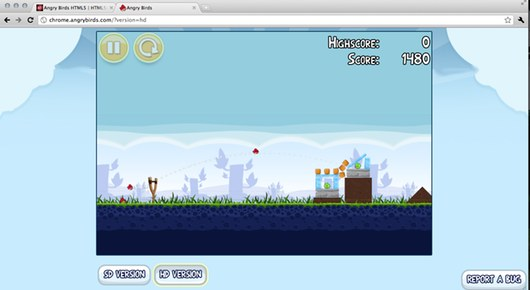
\includegraphics[height=\imgheight,width=\imgwidth]{angrybirds}
  \caption{Angry Birds {--} utilizando canvas em varias camadas}
  \label{img:angrybirds}
\end{figure}


\subsection{Transformações e transições com CSS3}

O CSS3 possui uma série de transformações e transições que permitem ao
desenvolvedor rotacionar e escalar os elementos de uma página
\cite{agi2011html5}. Apesar da grande movimentação dos desenvolvedores
em função do desenvolvimento de jogos utilizando as funcionalidades do
canvas, muito ainda é discutido sobre utilizar DOM para o
desenvolvimento de jogos, assim aproveitando as vantagens que o CSS3
pode trazer.
Uma das vantagens de ter um jogo que utiliza DOM ao invés de Canvas é
a maior compatibilidade com os navegadores, pois todos possuem suporte
a DOM, que é utilizado para a renderização das páginas de internet que
estão funcionando atualmente.

O CSS3 foi criado para suprir as necessidades de criações de efeitos
visuais para páginas de internet comuns, dando aos elementos DOM a
possibilidade de se transformar de várias maneiras. Ao ver essa nova
gama de funcionalidades algumas pesquisas foram feitas pelos
desenvolvedores para saber quais eram as vantagens de utilizá-las para
o desenvolvimento de jogos para o navegador.

As transições e transformações do CSS3 são muito úteis ao utilizar
objetos DOM para um jogo pois todos esses efeitos são renderizados
pelo navegador com aceleração de hardware, com isso ganhando
performance nos efeitos visuais.

Um exemplo de jogo feito com HTML5 e CSS3 utilizando transições e
transformações com CSS3 é o Anigma \cite{website:anigma}. Esse jogo
utiliza DOM para desenhar os objetos do jogo, javascript para
manipular suas posições e CSS3 para fazer os efeitos que fazem as
peças desaparecer ou rotacionar. Apesar de ser um jogo simples, o
Anigma é um ótimo exemplo para mostrar como o HTML5 pode ser utilizado
para a criação de jogos casuais por ser um jogo rápido, divertido e
relativamente simples.

\subsection{SVG}

SVG é uma linguagem de marcação utilizada para descrever aplicações de gráficos
bi-dimensionais e imagens, e um conjunto de scripts relacionados a
interfaces gráficas. \cite{website:w3csvg}. Essa linguagem é utilizada por
editores como o Inkscape para definir os vetores criados por ele.

Comparando SVG com Canvas, é possível verificar uma grande diferença
em termos de desenho. SVG é utilizado para construir desenhos
vetoriais que podem ser facilmente modificados, diferentemente do
canvas, que possui uma particularidade de não poder ser alterado, ou
seja, após um objeto canvas ser desenhado ele não pode ser mais
modificado, apenas redesenhado.

Com SVG também é possível fazer animações, assim possibilitando a
criação de mídias mais interativas, como logotipos animados e pequenas
animações de introdução.

Na Figura~\ref{img:timetrap}, é possível ver o logo da empresa
Timetrap, que foi desenvolvido apenas com SVG, utilizando animações. O
logo animado pode ser visto em \citeonline{website:svgtimetrap}.

\begin{figure}[H]
  \centering
	
\includegraphics[height=\imgheight,width=\imgwidth]{timetrap}
  \caption{Logo da empresa Timetrap {--} Utilizando apenas vetores SVG para sua construção}
  \label{img:timetrap}
\end{figure}

No desenvolvimento de jogos a utilização do SVG é bem limitada, sendo
comumente utilizada para as animações acima citadas. O motivo do SVG
não ser utilizado para o desenho dos jogos é a dificuldade e
performance de alterar cada um dos vetores, por esse motivo
a técnica de sprites é mais utilizada, favorecendo imagens pré-feitas
ao invés da manipulação de vetores.


\subsection{WebSocket API}

WebSocket API define uma especificação que permite às páginas web
utilizar o protocolo de Sockets para fazer comunicação em duas
vias com um servidor remoto. \cite{website:w3cwebsockets}. Com essa tecnologia
consegue-se facilmente criar jogos multiplayer, pois as informações
são trocadas entre dois computadores de uma maneira bem mais
veloz, trafegando menos dados e recebendo as informações mais
rapidamente.
O que traz essa velocidade na comunicação via internet é não utilizar
o método normal de comunicação que o HTTP fornece, e sim utilizar um
túnel direto entre o computador e o servidor.
Nos métodos normais de comunicação utilizando o HTTP a cada requisição
é necessário passar por todo o processo de comunicação do TCP, e
receber todos os dados e metadados do HTTP, o que gera um tempo maior para
o recebimento dos dados e um maior tráfego de rede. Com o Socket (que
é criado pela funcionalidade de WebSockets), apenas uma conexão TCP é
criada e mantida durante um período de tempo, assim facilitando o
tráfego de informações, viabilizando uma comunicação mais rápida e
adequada para um jogo em tempo real.

Websockets possibilita uma redução de 500 para 1 ou até 1000 para 1
(em alguns casos) de cabeçalhos de HTTP desnecessários, e até 3 para 1
em latência. \cite{lubbers2010pro}.

Na Figura~\ref{img:swarmation}, é apresentado um jogo que utiliza
uma biblioteca que disponibiliza uma interface de código Websockets.
A finalidade dela é tentar manter as mesmas interfaces em
todos os navegadores, inclusive os que não possuem suporte para essa
tecnologia. A ideia do jogo é integrar vários jogadores em um único lugar, sendo que
cada jogador assume o papel de um pixel, e eles precisam formar uma
determinada imagem que é gerada aleatoriamente pelo jogo e mostrada à
direita. A função do WebSockets nesse jogo é sincronizar em tempo real a
posição de cada jogador para saber ao final da contagem quais imagens
foram formadas e quais jogadores devem ser pontuados.

\begin{figure}[H]
  \centering
	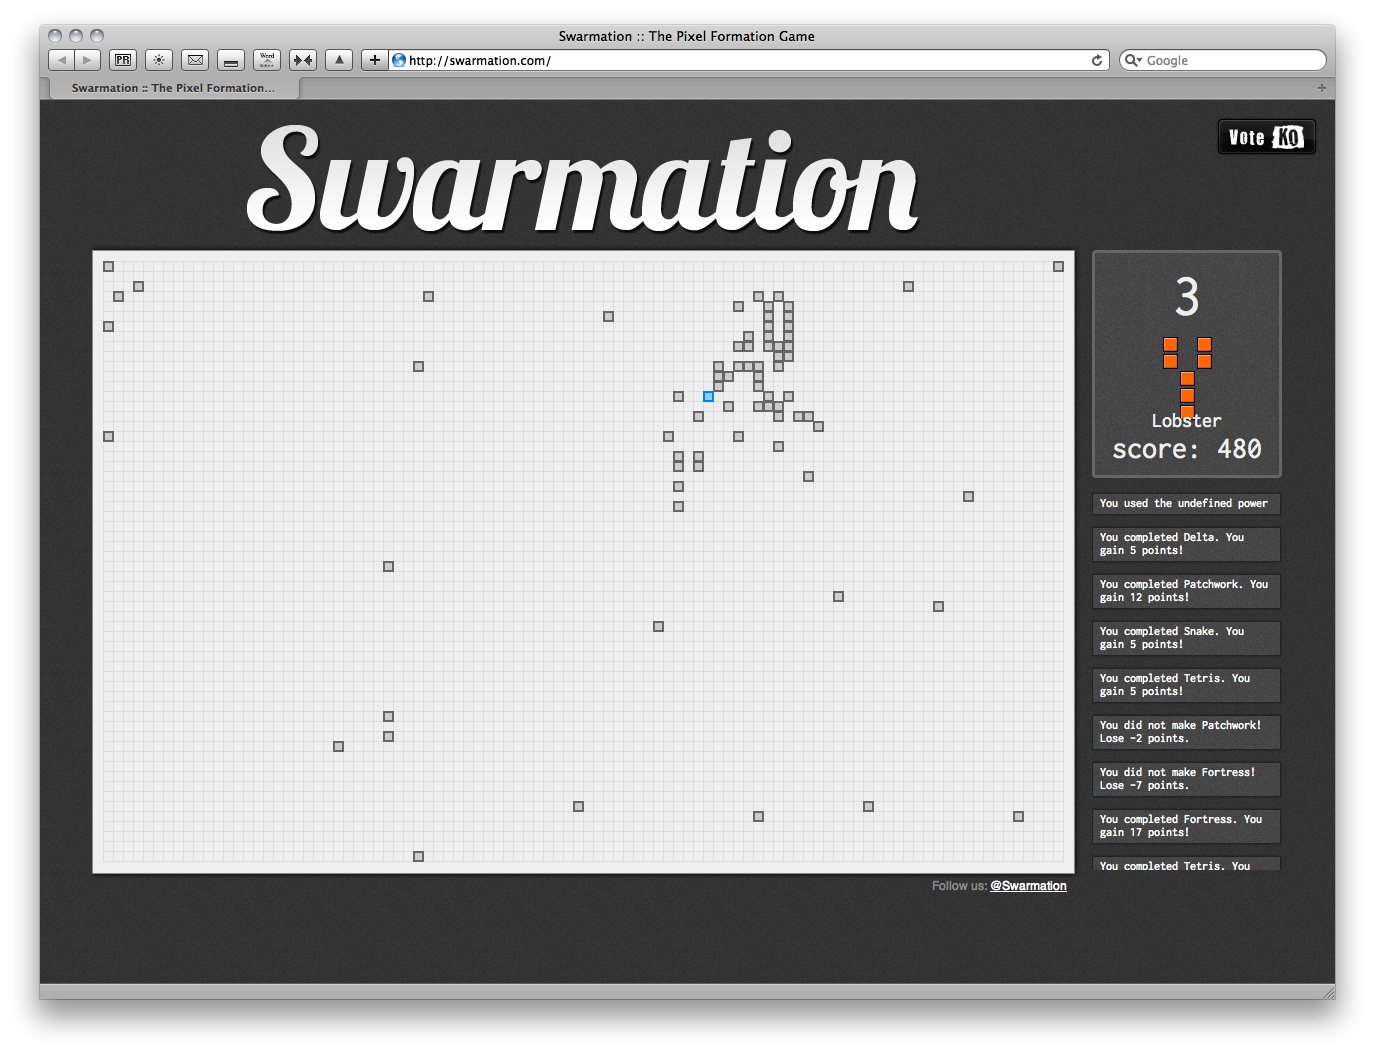
\includegraphics[height=\imgheight,width=\imgwidth]{swarmation}
  \caption{Swarmation {--} Jogo casual simples que utiliza Websockets}
  \label{img:swarmation}
\end{figure}


\subsection{Offline cache}

Offline cache, em sua maneira mais simplista, é uma lista apontando
para o HTML, CSS, scripts em Javascript, imagens e outros recursos que devem
estar disponíveis para o website. \cite{pilgrim2010html5}. O arquivo de
manifesto é o responsável por conter essa lista de arquivos, provendo
ao navegador a informação sobre os recursos que
precisam ser utilizados quando o dispositivo que está executando a
página em questão não estiver apto a acessar a internet, ou seja,
na primeira requisição, tudo que estiver disponível no arquivo de manifesto
que contém essa lista será baixado, guardado no dispositivo e utilizado até
que o manifesto seja modificado.

A cada nova requisição de uma aplicação que utiliza offline cache o
navegador verifica o arquivo de manifesto se ele não foi modificado
o navegador vai utilizar os arquivos que estão disponíveis localmente,
caso contrário todos os arquivos da seção "CACHE" desse arquivo serão baixados novamente.

A funcionalidade de offline cache também prevê os recursos que não
podem ser guardadas localmente e as que precisam
necessariamente estar online para funcionar corretamente, e para isso
existe uma seção chamada REMOTE no arquivo manifesto, definindo quais
são os arquivos que não devem ser considerados quando o usuário não
estiver offline.

Todos os arquivos utilizados na aplicação devem estar no arquivo de
manifesto; para os arquivos que não estarão disponíveis localmente há
uma seção chamada FALLBACK.

Utilizando Offline cache é possível criar uma aplicação para a
internet que funcione normalmente sem a necessidade do usuário estar
conectado. Um exemplo dessa funcionalidade foi feito na aplicação da
Figura~\ref{img:currency}. A aplicação em questão pode ser adicionada
no celular como um favorito (no caso do iPhone, pode ser adicionado
como um novo aplicativo à tela principal do aparelho) e ser utilizada
normalmente como se fosse uma aplicação nativa.

\begin{figure}[H]
  \centering
	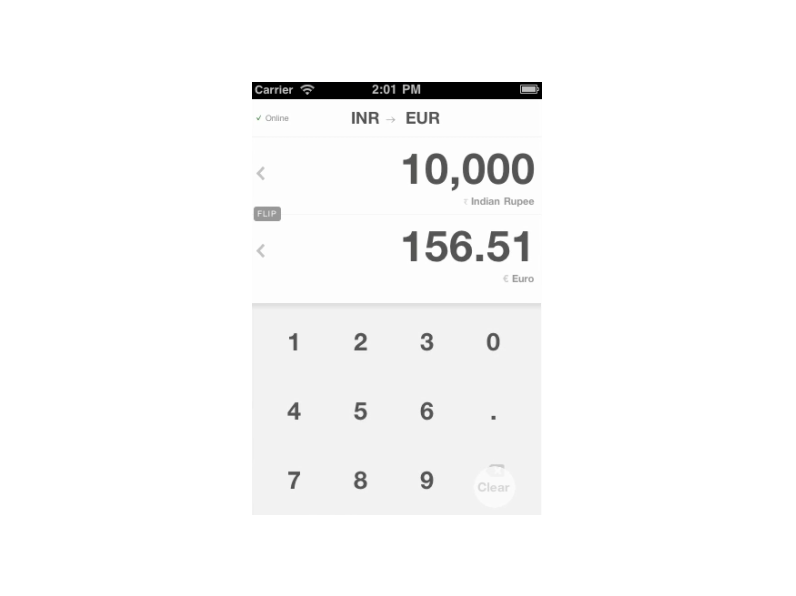
\includegraphics[height=\imgheight,width=\imgwidth]{currency}
  \caption{Offline cache {--} Currency.io utilizando offline cache
  para fazer uma aplicação que ficará disponível mesmo sem acesso a
  internet.}
  \label{img:currency}
\end{figure}

Essa funcionalidade pode ser muito utilizada em jogos casuais para
disponibilizar uma determinada aplicação para utilização em um
dispositivo móvel. No caso de um jogo, bastaria adiciona-lo aos favoritos,
e ele estará disponível a qualquer momento.


\subsection{Local Storage}

Local Storage do HTML5 provê aos websites uma maneira de guardar
informações e recuperá-las depois, utilizando um conceito similar aos
cookies, mas já pensando em um grande modelo de dados. \cite{pilgrim2010html5}.
Por muito tempo os desenvolvedores utilizaram cookies para guardar
informações sobre o website diretamente no navegador do usuário, e
essa tecnologia se provou muito ineficiente para uma quantidade um
pouco maior de dados, pois além de ser limitado para guardar informações,
os dados ficam trafegando pela rede em cada requisição, consumindo
banda, expondo os dados, e deixando as requisições mais lentas.

O Local Storage foi criado para resolver esses problemas, dando uma
interface simples para o desenvolvedor guardar dados de sua
aplicação diretamente no navegador do usuário. Para guardar tais dados
o desenvolvedor utiliza um banco que armazena dados seguindo um
esquema chave-valor, ou seja, uma chave como índice, associado a um
determinado valor, que será convertido para texto quando adicionado.

Essa funcionalidade é muito utilizada em conjunto com a funcionalidade
de offline cache, pois quando uma aplicação não possui conexão com a
internet é necessário utilizar Local Storage para guardar informações
que serão sincronizadas com o servidor assim que a aplicação possuir
conexão com a internet novamente.

Um exemplo que ilustra muito bem a utilização de Local Storage é a
aplicação do Google para visualização do Gmail offline (vide
figura~\ref{img:gmailoffline}), que utiliza Local Storage para guardar
as informações dos emails que ele controla, e utiliza offline cache
para manter a aplicação disponível sem a necessidade de conexão com a
internet.

\begin{figure}[H]
  \centering
	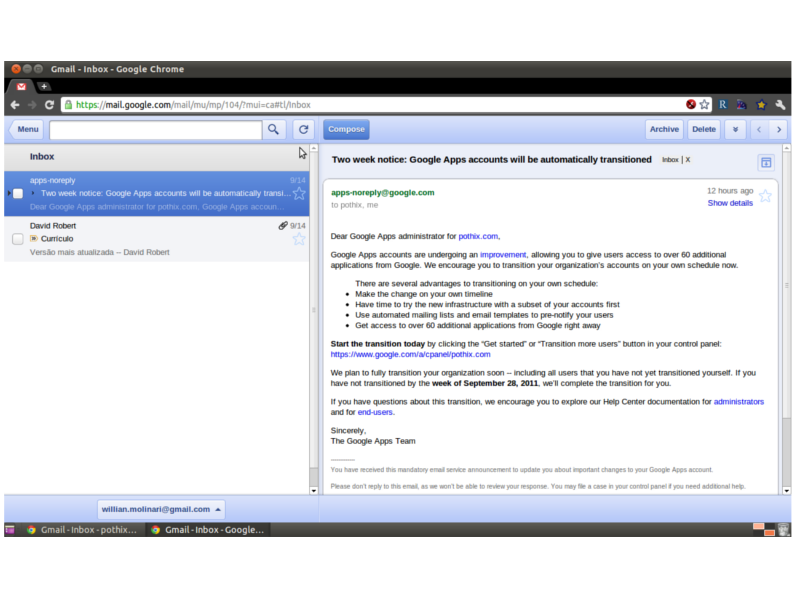
\includegraphics[height=\imgheight,width=\imgwidth]{gmailoffline}
  \caption{Offline cache {--} Aplicação do Gmail que possibilita a
  leitura dos e-mails offline com as mensagens sincronizadas
  previamente.}
  \label{img:gmailoffline}
\end{figure}

Utilizando essas funcionalidades para jogos casuais é possível
guardar informações de tabelas de pontos, nomes dos jogadores,
informações sobre os níveis e falas dos personagens durante o jogo e
etc. Quando a funcionalidade de offline cache for utilizada, local
storage provavelmente será utilizada em conjunto para manter a
consistência dos dados do jogador, e possibilitar uma possível
sincronização com um servidor externo assim que houver conexão com a
internet.

\subsection{Áudio}
Para suprir uma das necessidades multimídia
da internet foi a \tagaudio. Com o passar do tempo e o aumento no
numero de sites, os conteúdos da internet foram mudando
e se tornando cada vez mais multimídia, e não apenas hipertexto de
acordo com a ideia inicial. Para utilizar esse tipo de mídia na
internet foram utilizados componentes externos, como o Adobe Flash por
exemplo, pois a internet ainda não estava preparada para resolver esse
tipo de problema.

O padrão HTML5 define uma forma para adicionar áudio a uma página de
internet de uma maneira fácil e sem depender de produtos externos.
Isso é feito através da \tagaudio, que traz uma
implementação nativa (que será feita pelos navegadores) para que o
áudio seja executado.

Essa funcionalidade fornece uma API Javascript para a manipulação do
áudio inserido no documento, conforme
\citeonline{pfeiffer2010definitive}.
Com isso é possível parar, pausar, tocar,
pular entre várias partes do áudio, entre outras funcionalidades.

Um dos problemas que podem ser encontrados com a \tagaudio é o tipo de
implementação de formatos que cada navegador suporta. Há um exemplo
simples desse problema na atual data de escrita desse trabalho. O
navegador Firefox possui a implementação do formato \textit{ogg}, que
é um formato aberto, enquanto outros navegadores como o Chrome por
exemplo, implementam o formato \textit{mp3}. Esse problema pode ser
facilmente contornado pela implementação atual da \tagaudio,
apenas definindo os dois formatos na mesma tag permitindo que o
navegador escolha o arquivo correto para ser executado.

A apresentação do conteúdo associado à \tagaudio possui algumas particularidades que não permitem uma
resposta rápida e pode atrapalhar a jogabilidade provendo um som com
atraso. Para resolver esse problema está sendo desenvolvido a
Web Audio API, que fornece APIs bem parecidas com a \tagaudio, mas
tratando os eventos no momento certo, lidando com a taxa de
atualização de cada dispositivo.

\begin{figure}[H]
  \centering
	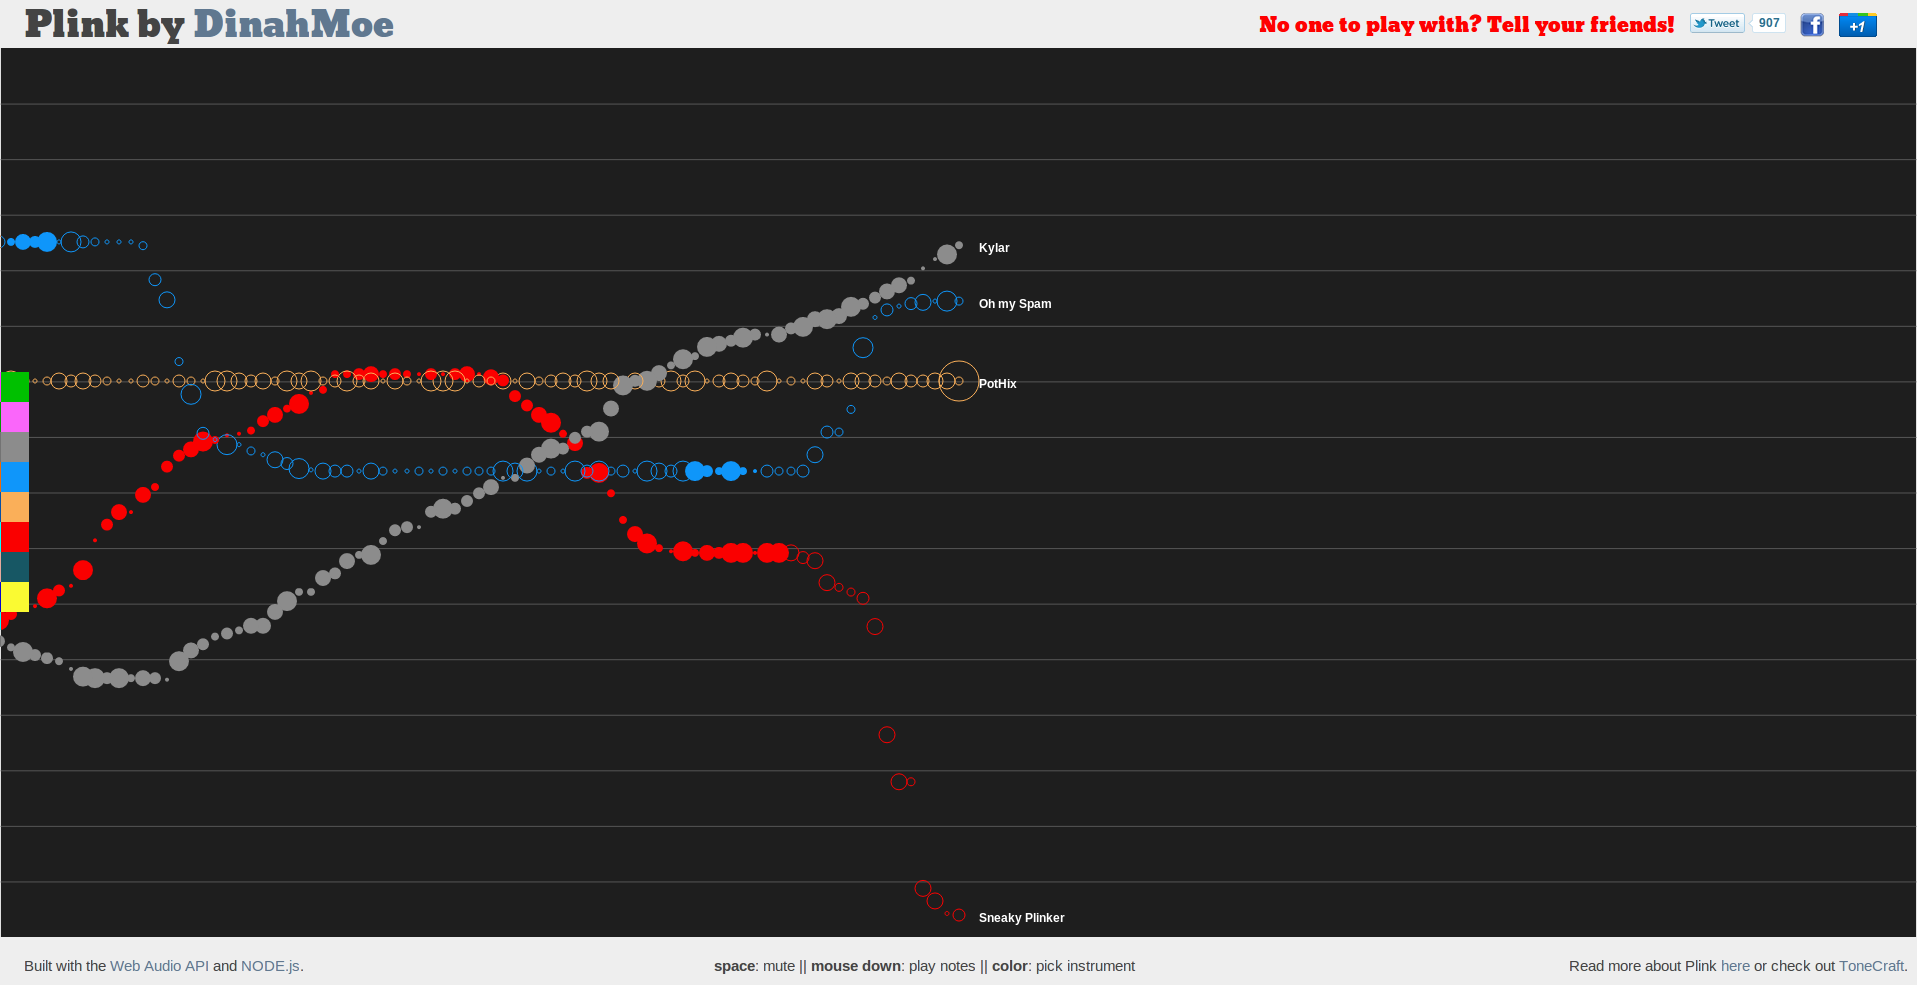
\includegraphics[height=\imgheight,width=\imgwidth]{webaudioapi}
  \caption{Plink {--} Jogo feito utilizando Web Audio Api}
  \label{img:webaudioapi}
\end{figure}

A Figura~\ref{img:webaudioapi} mostra o jogo Plink, que utiliza Web
Audio Api para fornecer aos usuários uma forma divertida de interagir
entre si e criar músicas. Cada usuário controla sua posição com o
mouse, e o som gerado depende da sua posição e cor. Esse é um ótimo
exemplo de como a Web Audio API está trazendo a manipulação de audio
em tempo real para o navegador, assim resolvendo os problemas de
latência da tag \textit{<audio>}.

Essas funcionalidades são muito úteis para o desenvolvimento de jogos, pois
todos os sons que o jogo deve produzir podem ser adicionados e
manipulados utilizando essas funcionalidades, assim criando uma
experiencia mais divertida para o jogador.

\subsection{WebGL}

Seguindo a definição de \citeonline{lubbers2010pro}, WebGL é uma API para gráficos 3D na web. Essa
API possibilita a criação de jogos que exigem mais processamento do
computador pois utiliza a GPU do dispositivo em questão para processar
os gráficos do jogo.

Essa tecnologia é baseada no OpenGL ES2, apenas um mapeamento para
Javascript conforme \citeonline{lubbers2010pro}, portanto possui
quase todas as funcionalidades que as versões para celular possuem,
inclusive shaders. Essa particularidade contribui
para que os atuais desenvolvedores de jogos (principalmente jogos em
três dimensões) tenham mais facilidade para portar os jogos mais
simples para web, apenas lidando com as particularidades de cada
navegador e com o fluxo diferenciado que um jogo web terá.

O WebGL é baseado na tag \textit{<canvas>}, e utiliza a mesma tag
empregada para fazer desenhos canvas comums, mas ao invés de utilizar o contexto
2D, é utilizado o contexto 3D.

Um dos possíveis problemas de se utilizar WebGL na atual data
de escrita desse trabalho é a falta de suporte dos navegadores e
dispositivos para essa funcionalidade. Como o WebGL depende muito do
hardware do dispositivo, dar suporte para ele ainda é um problema,
pois depende dos drivers de cada dispositivo funcionar
corretamente, além do navegador possuir suporte para o mesmo.
WebGL está sendo bem utilizado atualmente para acelerar a execução do jogo,
mas sem depender totalmente dele para que o jogo funcione, assim
aproveitando as vantagens do WebGL para os navegadores e sistemas que
possuem esse suporte.

Na Figura~\ref{img:webglmodels} é possível ver modelos 3D no formato
MD2 (o mesmo formato que o jogo Quake II utilizava para seus
personagens) utilizando WebGL para a renderização. Isso é feito utilizando a
biblioteca GLGE, que é um facilitador para a utilização do WebGL.

\begin{figure}[H]
  \centering
	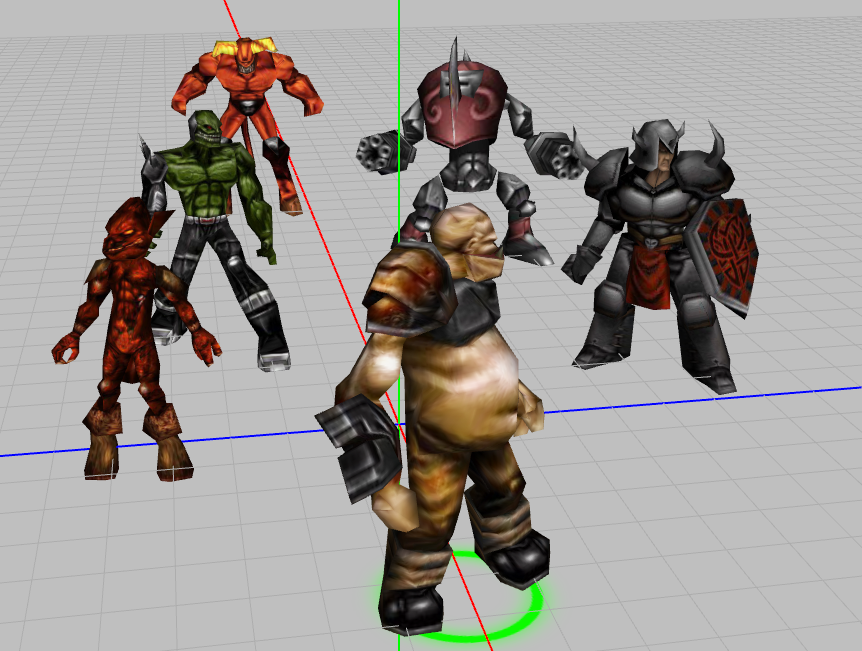
\includegraphics[height=\imgheight,width=\imgwidth]{webglmodels}
  \caption{Modelos 3D {--} Modelos de personagens 3D sendo renderizados com WebGL}
  \label{img:webglmodels}
\end{figure}

A figura~\ref{img:webglmodels} dá uma ideia de para onde o WebGL está
caminhando, e provavelmente daqui a algum tempo será possível criar
jogos 3D simples que funcionarão diretamente no navegador, ou seja,
é possível que os jogos simples em três dimensões que estão atualmente
disponíveis para celulares sejam desenvolvidos novamente para
serem executados diretamente no navegador num futuro não tão distante.

Outro exemplo de como WebGL pode ser poderoso pode ser visto na
Figura~\ref{img:webglwater},
que está disponível integralmente em \citeonline{website:webglwater}.
Nesse exemplo 3D são utilizadas várias técnicas de sombreamento e
manipulação da água e da iluminação, que exigem um bom processamento
do dispositivo, e o WebGL desempenha um ótimo papel em computadores
modernos.

\begin{figure}[H]
  \centering
	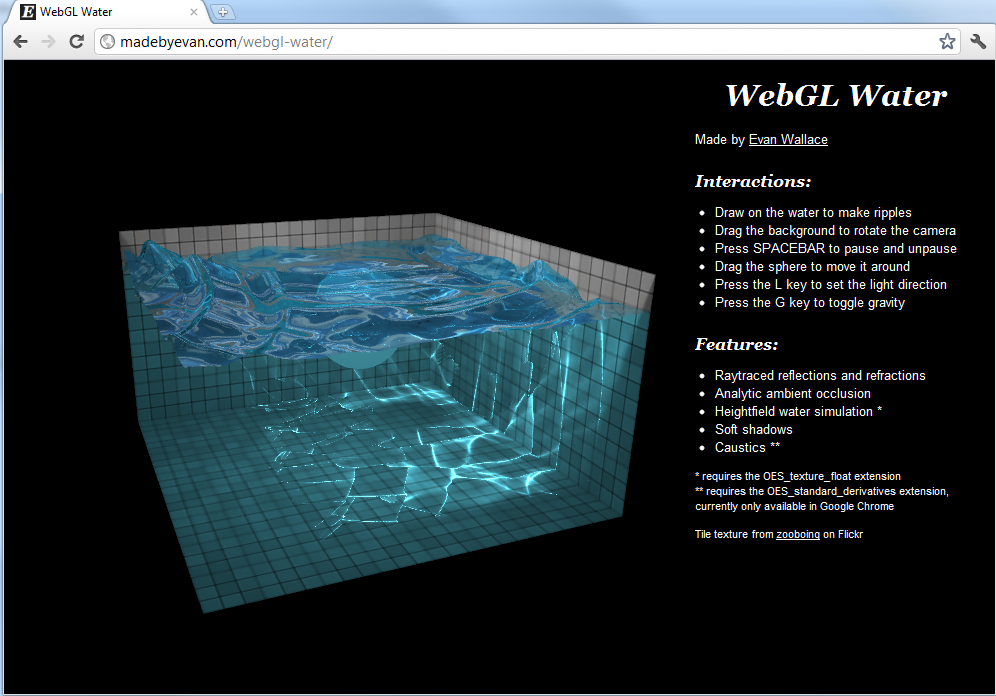
\includegraphics[height=\imgheight,width=\imgwidth]{webglwater}
  \caption{WebGL Water {--} Utilizando o processamento para obter
  bonitas cenas em 3D}
  \label{img:webglwater}
\end{figure}

Apesar de bonitos e interessantes, esses exemplos são apenas provas de
conceito para mostrar que o WebGL é realmente útil e pode ser
utilizado para aplicações que exijam um grande processamento do
navegador. Mas além de provas de conceito, alguns jogos já estão
utilizando WebGL como tecnologia auxiliar para acelerar no desenho dos
gráficos e nos cálculos.
Na Figura~\ref{img:emberwind} é possível ver um exemplo do jogo Emberwind
sendo executado utilizando WebGL.

\begin{figure}[H]
  \centering
	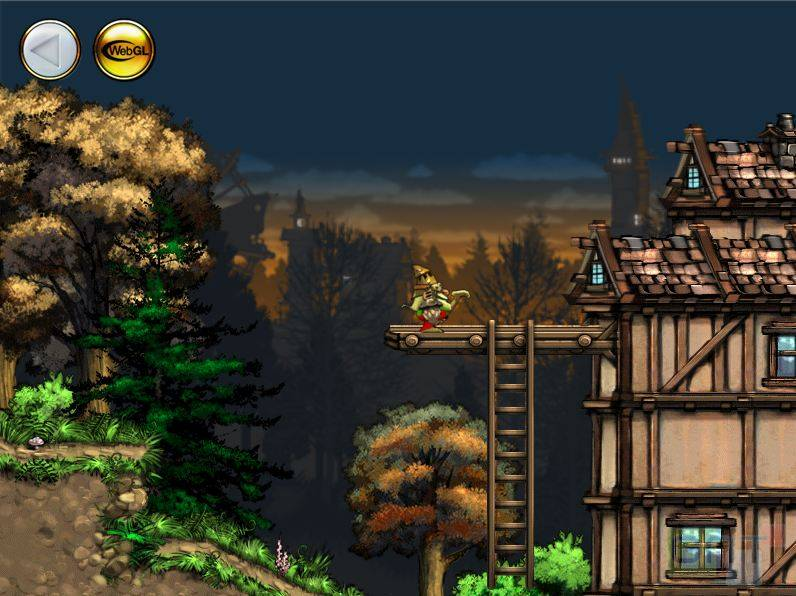
\includegraphics[height=\imgheight,width=\imgwidth]{emberwind}
  \caption{Emberwind {--} Utilizando o poder do WebGL para acelerar o processamento}
  \label{img:emberwind}
\end{figure}

Esse jogo em particular está sendo portado para a plataforma web,
fortificando o argumento dado neste subcapítulo. Uma particularidade
desse jogo é a opção de se utilizar apenas canvas para os dispositivos
que não suportam WebGL, o que mostra que é possível contornar a falta
de suporte do WebGL para jogos casuais nos dispositivos atuais, assim
como foi dito previamente.

\clearpage

  \section{Comparação com as tecnologias atuais}

Com base nas funcionalidades apresentadas sobre as tecnologias que
fazem parte da especificação do HTML5, será feita uma comparação com
as principais ferramentas utilizadas para o desenvolvimento de jogos
na data da escrita desse trabalho.

\subsection{Tecnologias atuais}

As ferramentas atuais para desenvolvimento de jogos para a internet se
utilizam de extensões que são instaladas nativamente no computador
para que possa ser uma plataforma na qual o jogo desenvolvido vai
executar sobre, para assim gerar uma plataforma mais consistente para
o desenvolvimento e ter um melhor acesso ao hardware do dispositivo em
questão. Essas tecnologias são:

\subsubsection{Java}

Java foi uma das primeiras tecnologias a ser aplicadas sobre os
navegadores, logo após a criação do Java, quando a tecnologia foi
portada uma facil execução sobre o navegador utilizando os chamados
applets.
%TODO: Escrever mais sobre os applets e sua utilização

\subsubsection{Flash}

Flash é um produto da Adobe para enriquecer a o visual de uma página
de internet, trazendo conteúdo multimídia. Atualmente, o Flash é a
tecnologia mais utilizada para desenvolvimento de jogos para a
internet, tendo sua extensão instalada em mais de 90 por cento dos
computadores pessoais.

%FIXME: Achar algumas referencias do flash como produto mais utilizado
%FIXME: Achar algumas referencias do flash com seu plugin instalado em mais de 90% dos navegadores
%TODO: Escrever mais sobre o flash

\subsubsection{Unity}

É uma tecnologia nova que está ganhando muito espaço no mercado de
desenvolvimento de jogos. Essa engine exporta o jogo desenvolvido para
diversas plataformas, entre elas o navegador, que utiliza um plugin um
plugin para executa-lo, assim como as tecnologias anteriores.
Uma das grandes vantagens dessa tecnologia é a facilidade para se
fazer jogos, pois esse é o foco da engine.

%TODO: Pesquisar mais sobre a Unity para dar uma visão mais ampla

\subsection{Performance}

No mundo dos jogos digitais, performance é um assunto muito falado,
pois os jogos consomem muito recurso do dispositivo em que estão
executando, pois estão, entre outras coisas, em constante execução, fazendo
calculos diversos para situar o jogador dentro do jogo, por exemplo.
Entre esses calculos, dependendo do jogo, estão calculos de fisica dos
objetos da cena e do próprio jogador, transformação de imagens para
dar impressão de movimento ou sombra e outras coisas que exigem alto
processamento em um curto período de tempo.
As tecnologias Java, Flash e Unity possuem uma performance melhor no
momento de escrita desse trabalho, pois eles possuem seu próprio
software desenvolvido, e roda nativamente no sistema operacional,
assim ganhando várias vantagens como um processo separado no sistema,
apenas executando um jogo que foi préviamente "compilado"
especialmente para essa tecnologia.

O HTML5 juntamente com Javascript perde um pouco em performance, pois
o sistema operacional vê apenas um navegador como processo, e esse
navegador vai fazer a interface entre o jogo e o sistema operacional.
Temos que levar em consideração que o navegador também tem seus
"processos" (outras páginas de internet que podem estar abertas no
momento), e ele deve gerenciá-las da melhor maneira.

%TODO: Continuar escrevendo essa parte, ainda está pela metade

\subsection{Portabilidade}

Lorem ipsum dolor sit amet, consectetur adipisicing elit, sed do eiusmod tempor incididunt ut labore et dolore magna aliqua. Ut enim ad minim veniam, quis nostrud exercitation ullamco laboris nisi ut aliquip ex ea commodo consequat. Duis aute irure dolor in reprehenderit in voluptate velit esse cillum dolore eu fugiat nulla pariatur.  Excepteur sint occaecat cupidatat non proident, sunt in culpa qui officia deserunt mollit anim id est laborum

\subsection{Fragmentação}

Lorem ipsum dolor sit amet, consectetur adipisicing elit, sed do eiusmod tempor incididunt ut labore et dolore magna aliqua. Ut enim ad minim veniam, quis nostrud exercitation ullamco laboris nisi ut aliquip ex ea commodo consequat. Duis aute irure dolor in reprehenderit in voluptate velit esse cillum dolore eu fugiat nulla pariatur.  Excepteur sint occaecat cupidatat non proident, sunt in culpa qui officia deserunt mollit anim id est laborum

\subsection{Recursos para desenvolvimento}

Lorem ipsum dolor sit amet, consectetur adipisicing elit, sed do eiusmod tempor incididunt ut labore et dolore magna aliqua. Ut enim ad minim veniam, quis nostrud exercitation ullamco laboris nisi ut aliquip ex ea commodo consequat. Duis aute irure dolor in reprehenderit in voluptate velit esse cillum dolore eu fugiat nulla pariatur.  Excepteur sint occaecat cupidatat non proident, sunt in culpa qui officia deserunt mollit anim id est laborum

  \section{Considerações finais}
%TODO: Escrever um pouco mais sobre esse tópico

Após analisar HTML5 como tecnologia para desenvolvimento de jogos para
a internet, utilizando os navegadores em seu atual estado de
desenvolvimento e comparando com as principais ferramentas utilizadas
para desenvolvimento até o momento, é possível se concluir que é
totalmente viável o desenvolvimento de um jogo casual simples
utilizando HTML5 e Javascript como tecnologia.

Levando em consideração as funcionalidades do HTML5 como Canvas para o
desenho de objetos na tela, o Offline cache para manter um jogo
disponível sem a necessidade de uma conexão com a internet, o Local
Storage para guardar informações sem a nacessidade de trafegá-las em
cada requisição, os Websockets para fazer jogos multiplayer utilizando
uma conexão consistente, e todas as outras vantagens que foram
explicadas em mais detalhes durante o decorrer do trabalho,
é fácil perceber que os navegadores estão preparados para
receber jogos que exigem apenas cálculos relativamente
simples, como física básica e posicionamentos dos personagens, que é
praticamente o que é utilizado para se fazer um jogo simples. E aos
poucos os navegadores vão recebendo funcionalidades e otimizações para
lidar com jogos mais complexos, e também para melhorar a performance
dos jogos já desenvolvidos.

HTML5 é um conjunto de funcionalidades que visa melhorar o conteúdo
atual da internet sem a necessidade de ferramentas de terceiros, é uma
tecnologia nova que vem atender uma demanda conhecida da
internet mundial, e está assumindo esse papel muito bem, cada vez mais
ganhando publico e mostrando que realmente consegue atender a demanda
que foi criado para atender.

Desenvolver jogos em HTML5 atualmente é
apostar no futuro da tecnologia, utilizando o que já está
desenvolvido, que é o suficiente para se fazer jogos simples, e
acompanhar a evolução do mesmo, desenvolvendo novas funcionalidade
conforme elas vão sendo desenvolvidas pelos navegadores, assim se
tornando referência na área de desenvolvimento de jogos com uma
tecnologia nova que irá revolucionar o mercado.

Algumas empresas tem apostado nessa tecnologia, aproveitando
principalmente a vantagem de ter seu conteúdo disponível em
dispositivos móveis que não suportam outras tecnolovias de terceiros
como Java, Flash e etc. Aos poucos a própria Adobe está investindo em
HTML5, criando novas ferramentas para ajudar
os desenvolvedores \cite{website:adobeedge}, e até mesmo fazendo
demonstrações e experiências para mostrar as capacidades do HTML5 como
plataforma para aplições RIA, também conhecidas como aplicações ricas
para internet.

\subsection{Vantagens do HTML5}
Após as comparações é possível chegar a uma conclusão sobre quais são
as vantagens do HTML5 sobre as tecnologias que são utilizadas
atualmente.

Uma das vantagens claras que atrapalham muito os desenvolvedores de
jogos atualmente é a portabilidade, pois os desenvolvedores muitas
vezes precisam traduzir seu código para um grande quantidade de
plataformas para poder atingir uma quantidade maior de jogadores. O
problema com esse modelo é a fragmentação que isso gera, pois o mesmo
código estará dividido entre várias plataformas, com várias linguagens
de programação e provavelmente várias equipes de trabalho para manter
o jogo funcionando e corrigir cada problema que apareça. Quando um
problema é detectador na parte padrão do jogo todas as equipes devem
ser informadas e todos devem fazer determinada alteração e publicar o
jogo novamente para a plataforma que o jogo está executando.

Utilizando HTML5 esse problema é resolvido com facilidade, pois caso
um problema seja encontrado na parte padrão do jogo, ele vai ser
corrigido no jogo principal e enviado para o ambiente de produção, com
isso todos os jogadores terão o jogo atualizado assim que acessarem o
jogo em um navegador com conexão com a internet. Isso facilita muito a
distribuição dos jogos, apenas cabendo ao desenvolvedor tratar os
tamanhos de telas e dispositivos de entrada no seu jogo.

\subsection{Desvantagens do HTML5}
Assim como toda tecnologia o HTML5 também possui suas desvantagens
sobre seus concorrentes, e muitas vezes as vantagens se tornam
desvantagens dependendo do ponto de vista do desenvolvedor.

A vantagem de se ter apenas um código para todas as plataformas é
considerada desvantagem por alguns desenvolvedores, pois dessa maneira
muitas condições devem ser tratadas para que o jogo funcione bem em
todas as plataformas, e isso torna o código difícil de ser mantido
dependendo de como o desenvolvedor organizá-lo.
Esse mesmo problema acontece com desenvolvedores de aplicações para o
sistema operacional Android, que precisam tratar as diferentes
configurações de \textit{hardware} de cada dispositivo, suas
velocidades de processamento, tamanho de tela e etc. Alguns
desenvolvedores (como é o caso da Rovio, criadora do jogo Angry Birds)
decidiram fazer diversos jogos para diversos aparelhos para evitar
esse tipo de fragmentação.

\subsection{Sugestões para pesquisas futuras}

Este trabalho visou mostrar as vantagens e desvantagens de se utilizar
HTML5 e Javascript para desenvolver jogos casuais para o navegador,
para dar uma visão geral do que a plataforma é capaz de fazer, e quais
os problemas que devem ser evitados comparando-os com as tecnologias
que são utilizadas atualmente para tal finalidade.

O conteúdo desse trabalho não é focado em partes específicas do
desenvolvimento de jogos para poder dar uma visão geral da plataforma.
Há muito há ser pesquisado sobre as várias áreas mencionadas nesse
trabalho, Entre os vários assuntos que podem extender esse trabalho
estão:

Como obter lucro com desenvolvimento de jogos em HTML5, quais as vantagens
e desvantagens que a plataforma pode oferecer para essa
finalidade. Este trabalho não cobre esse tema pois muito deve ser
pesquisado sobre propaganda e como aplica-la de uma maneira a ser
melhor aproveitada em um jogo casual, além do estudo dos melhores
meios de venda de jogos para a internet e a disponibilização de
serviços para conseguir tal renda do jogador.

Desenvolvimento de jogos com HTML5 focado em dispositivos móveis, como
obter performance, utilizar uma banda limitada e menor consumo de
bateria. Este trabalho não cobre esse tema pois isso requer uma maior
pesquisa sobre o hardware dos dispositivos móveis e suas limitações,
estudos de performance a fundo para mostrar como conseguir um menor
custo de processamento, assim reduzindo o consumo de bateria, entre
outras coisas que fariam com que esse trabalho tomasse um enfoque
diferente.

  \addcontentsline{toc}{section}{Referências}

\renewcommand{\refname}{\section*{Referências}}
\bibliography{bibliografia}
\newpage

  \addcontentsline{toc}{section}{GLOSSÁRIO}

\section*{Glossário}

\begin{description}
\item[3G ] Terceira geração de tecnologias de acesso móvel, hoje
bastante conhecida por fornecer conexão com a internet.
\item[Android ] Sistema operacional para dispositivos móveis criado
pelo Google, possui um navegador que suporta vários recursos do HTML5.
\item[DOM ] Document Object Model, ou modelo de objeto de documentos,
é uma especificação da W3C onde é possível editar a estrutura
dinamicamente. Essa especificação possui uma interface padrão para
acesso aos elementos do documento, facilitando a manipulação dos
elementos individualmente.
\item[Driver ] Software que provê ao sistema operacional uma forma
fácil de lidar com um determinado hardware.
\item[Eclipse ] É uma ferramenta para desenvolvimento de software, uma
IDE (Integrated Development Environment, ou Ambiente de
desenvolvimento integrado).
\item[IETF ] Internet Engeenering Task Force
\item[iPhone ] Dispositivo móvel criado pela Apple, possui o iOS como
sistema operacional e um navegador que suporta vários recursos do HTML5.
\item[Engine ] Software de auxílio ao desenvolvimento de jogos. Provê
uma boa interatividade com o desenvolvedor, utilizando uma interface
gráfica para adicionar imagens, texturas e macros para o jogo.
\item[Flash Player ] É a ferramenta da adobe que executa projetos
feitos com o Flash
\item[FPS ] Frames por segundo, é a taxa de atualizacão que um jogo
consegue atingir. O que essa taxa mostra é quantas vezes o jogo
consegue fazer atualizacões na tela em um segundo. A quantidade padrão
utilizada para jogos é de 60 frames por segundo, ou seja, 60 fps.
\item[HTML ] HyperText Markup Language, a linguagem de marcação
utilizada para descrever as páginas de internet atualmente.
\item[HTTP ] HyperText Transfer Protocol, ou protocolo de
transferencia de hypertexto, é uma das principais tecnologias
utilizadas na internet. Esse protocolo é utilizado para enviar páginas
entre um servidor e um cliente.
\item[Inkscape ] É um editor de gráficos vetoriais de código aberto
utilizado para fazer desenhos vetoriais.
\item[IO ] Input/Output, entrada e saída, ou seja, trafego de dados.
\item[Java Applets ] Um Applet é um programa escrito em Java que pode
ser incluído em uma página HTML.Quando um navegador com suporte a
tecnologia Java acessa uma página com um applet, o código Java é
transferido para o computador do usuário e executador pela JVM do
navegador.
\item[JVM ] Java Virtual Machine, ou maquina virtual do Java, é a
maquina virtual que executa os softwares pré-compilados, escritos em
Java.
\item[plugin ] É um software externo que complementa outro software já
instalado.
\item[RIA ] Rich Internet Applications, ou aplicações ricas para
internet, são aplicações que possuem muito conteúdo multimídia e que
dão uma sensação diferente ao usuário, não parecem uma página web
comum.
\item[Sprite ] É uma imagem que define um conjunto de imagens que
serão utilizadas dentro do jogo. Essa imagem é mapeada para que apenas
mudando as posições dentro do jogo outra imagem possa ser mostrada,
dando assim a sensação de movimento ao jogador.
\item[TCP ] Transmission Control Protocol, ou Protocolo de Controle de
Transmissão, é uma dos protocolos mais utilizados em redes de
computadores, e seu trabalho é garantir que o pacote vai chegar até o
seu destino.
\item[WYSIWYG ] What You See Is What You Get, ou O que você vê é o que
você obtem. Significa a capacidade de um programa de computador de
permitir que um documento, enquanto manipulado na tela, tenha a mesma
aparência de sua utilização, usualmente sendo considerada final a
forma impressa.
\item[W3C ] World Wide Web Consortium, ou o Consórcio World Wide Web,
é um consórcio internacional, no qual seus filiados (empresas e
pessoas físicas) trabalham juntos para desenvolver padrões para a
internet.
\item[XHTML ] eXtensible Hypertext Markup Language.
\item[XML ] eXtensible Markup Language.

\end{description}
\newpage

  \appendix
\renewcommand{\appendixtocname}{Ap�ndices}
\renewcommand{\appendixpagename}{Ap�ndices}

\section{Question�rio}

Esta pesquisa tem por objetivo avaliar o grau de ader�ncia
desta empresa �s recomenda��es de seguran�a da
informa��o da norma internacional ISO/ IEC 17799:2001. Deste
modo, para ter dados referenciais da sua organiza��o, gostaria de
contar com sua colabora��o respondendo �s quest�es abaixo.

Esta pesquisa � de cunho cient�fico, tendo como premissa �
preserva��o da confidencialidade das informa��es. Esta
�, tamb�m, uma boa oportunidade para avaliar o controle de
\SI da sua empresa, pois respondendo este
question�rio, voc� receber� o �ndice de conformidade de sua
empresa com esta norma ISO 17799, de acordo com o escopo desta
pesquisa. \\

\hspace{-2cm}Obrigada! \\
\newlength{\tabquestwidth}
\setlength{\tabquestwidth}{7cm}

\hspace{-2cm}\begin{tabularx}{\textwidth}{|X|}
  \hline
  \tabitem INFORMA��ES SOBRE O RESPONDENTE \\
  \hline
  Cargo: \\
  Efetivo ( \ ) \ \ Terceiro ( \ ) \\
  \hline
\end{tabularx}

\bigskip

\hspace{-2cm}\begin{tabularx}{\textwidth}{|p{\tabquestwidth}|X|X|X|X|X|}
  \hline
  \multicolumn{6}{|l|}{\tabitem POLITICA DE SEGURAN�A} \\
  \hline
  \cabecalhotabela
  \hline
  \cellitem A organiza��o possui uma pol�tica de Seguran�a da Informa��o
           (SI) atualizada.\fimcel
  \hline
  \cellitem H� na organiza��o algu�m respons�vel pela gest�o da pol�tica de
            SI, com capacidade para realizar esta fun��o. \fimcel
  \hline
  \cellitem Existe documento atualizado que formaliza a pol�tica de SI
            aprovado pela dire��o, publicado e comunicado de forma adequada
            para todos os integrantes da organiza��o. \fimcel
  \hline
\end{tabularx}

\bigskip

\hspace{-2cm}\begin{tabularx}{\textwidth}{|p{\tabquestwidth}|X|X|X|X|X|}
  \hline
  \multicolumn{6}{|l|}{\tabitem SEGURAN�A ORGANIZACIONAL} \\
  \hline
  \cabecalhotabela
  \hline
  \cellitem A organiza��o possui uma infra-estrutura atualizada de SI para
            gerenciar a��es corporativas. \fimcel
  \hline
  \cellitem A organiza��o possui um f�rum de seguran�a ativo, formado pelo
            corpo diretor, a fim de gerir mudan�as estrat�gicas. \fimcel
  \hline
  \cellitem Existe uma defini��o clara e atualizada das atribui��es de
            responsabilidades associadas � SI. \fimcel
  \hline
  \cellitem Existe uma norma atualizada de identifica��o dos riscos no acesso
            dos prestadores de servi�os. \fimcel
  \hline
  \cellitem Existe um controle de acesso especifico para prestadores de
            servi�os de acordo com padr�es atuais. \fimcel
  \hline
\end{tabularx}

\bigskip


\hspace{-2cm}\begin{tabularx}{\textwidth}{|p{\tabquestwidth}|X|X|X|X|X|}
  \hline
  \multicolumn{6}{|l|}{\tabitem CLASSIFICA��O E CONTROLE DOS ATIVOS DE
                                INFORMA��O} \\
  \hline
  \cabecalhotabela
  \hline
  \cellitem Existe na organiza��o, invent�rio atualizado dos ativos f�sicos,
            tecnol�gicos e humanos. \fimcel
  \hline
  \cellitem Existe crit�rios de sigilo,atualizados, para classificar
           a informa��o. \fimcel
  \hline
\end{tabularx}

\bigskip

\hspace{-2cm}\begin{tabularx}{\textwidth}{|p{\tabquestwidth}|X|X|X|X|X|}
  \hline
  \multicolumn{6}{|l|}{\tabitem SEGURAN�A EM PESSOAS} \\
  \hline
  \cabecalhotabela
  \hline
  \cellitem Existem na organiza��o crit�rios atualizados de sele��o e pol�tica
  de recursos humanos. \fimcel
  \hline
  \cellitem Na contrata��o s�o previstos, de forma clara, acordo de
  confiabilidade, termos e condi��es de trabalho. \fimcel
  \hline
  \cellitem Existem processos atualizados para capacita��o e treinamento de
  usu�rios. \fimcel
  \hline
  \cellitem Existe uma estrutura atualizada para notificar e responder aos
  incidentes e falhas de seguran�a. \fimcel
  \hline
\end{tabularx}

\bigskip

\hspace{-2cm}\begin{tabularx}{\textwidth}{|p{\tabquestwidth}|X|X|X|X|X|}
  \hline
  \multicolumn{6}{|l|}{\tabitem SEGURAN�A F�SICA E DE AMBIENTE} \\
  \hline
  \cabecalhotabela
  \hline

  \cellitem Existe na organiza��o uma defini��o adequada de per�metros e
  controles de acesso f�sico aos diversos ambientes. \fimcel
  \hline
  \cellitem Existem recursos atualizados de seguran�a e manuten��o dos
            equipamentos. \fimcel
  \hline
  \cellitem Existe uma estrutura, atualizada, para o fornecimento adequado de
            energia. \fimcel
  \hline
  \cellitem Existe seguran�a no cabeamento da organiza��o, seguindo padr�es
            atuais. \fimcel
  \hline

\end{tabularx}

\bigskip

\hspace{-2cm}\begin{tabularx}{\textwidth}{|p{\tabquestwidth}|X|X|X|X|X|}
  \hline
  \multicolumn{6}{|l|}{\tabitem GERENCIAMENTO DAS OPERA��ES E COMUNICA��ES} \\
  \hline
  \cabecalhotabela
  \hline

  \cellitem S�o previstos na organiza��o procedimentos e responsabilidades
            operacionais atualizados. \fimcel
  \hline
  \cellitem Existe um controle atualizado de mudan�as operacionais. \fimcel
  \hline
  \cellitem Existe segrega��o de fun��o e ambientes atualizadas. \fimcel
  \hline
  \cellitem Existe planejamento e aceita��o dos sistemas seguindo padr�es
            atuais. \fimcel
  \hline
  \cellitem Existem procedimentos atualizados para realiza��o de c�pias de
            seguran�a. \fimcel
  \hline
  \cellitem Existem controles de gerenciamento de rede atualizados. \fimcel
  \hline
  \cellitem Existem procedimentos de seguran�a, atualizados, na documenta��o
            de sistemas. \fimcel
  \hline
  \cellitem S�o previstos mecanismos de seguran�a atuais para o correio
            eletr�nico. \fimcel
  \hline

\end{tabularx}

\bigskip

\hspace{-2cm}\begin{tabularx}{\textwidth}{|p{\tabquestwidth}|X|X|X|X|X|}
  \hline
  \multicolumn{6}{|l|}{\tabitem CONTROLE DE ACESSO} \\
  \hline
  \cabecalhotabela
  \hline

  \cellitem Existem na organiza��o normas atualizadas para o controle de
            acesso. \fimcel
  \hline
  \cellitem Existe gerenciamento de acesso de usu�rios atualizado. \fimcel
  \hline
  \cellitem Existe controle de acesso ao sistema operacional de acordo padr�es
            atuais. \fimcel
  \hline
  \cellitem Existe controle de acesso �s aplica��es de acordo com  padr�es
            atuais. \fimcel
  \hline
  \cellitem Existe monitora��o do uso e acesso aos sistemas de acordo com
            padr�es atuais. \fimcel
  \hline
  \cellitem S�o previstos crit�rios atualizados para computa��o m�vel e
            trabalho remoto. \fimcel
  \hline

\end{tabularx}

\bigskip

\hspace{-2cm}\begin{tabularx}{\textwidth}{|p{\tabquestwidth}|X|X|X|X|X|}
  \hline
  \multicolumn{6}{|l|}{\tabitem DESENVOLVIMENTO E MANUTEN��O DE SISTEMAS} \\
  \hline
  \cabecalhotabela
  \hline

  \cellitem Existem requisitos de seguran�a atualizados para os sistemas de
            informa��o. \fimcel
  \hline
  \cellitem Existem na organiza��o controles de criptografia atualizados.
            \fimcel
  \hline
  \cellitem S�o previstos mecanismos de seguran�a no processo de
            desenvolvimento e suporte, de acordo com padr�es atuais. \fimcel
  \hline

\end{tabularx}

\bigskip

\hspace{-2cm}\begin{tabularx}{\textwidth}{|p{\tabquestwidth}|X|X|X|X|X|}
  \hline
  \multicolumn{6}{|l|}{\tabitem GEST�O DA CONTINUIDADE DO NEGOCIO} \\
  \hline
  \cabecalhotabela
  \hline
  \cellitem Existe na organiza��o um processo atualizado de gest�o da
            continuidade do neg�cio. \fimcel
  \hline
  \cellitem A organiza��o realiza testes, manuten��o e reavalia��o do plano de
            continuidade do negocio regularmente. \fimcel
  \hline

\end{tabularx}

\bigskip

\hspace{-2cm}\begin{tabularx}{\textwidth}{|p{\tabquestwidth}|X|X|X|X|X|}
  \hline
  \multicolumn{6}{|l|}{\tabitem CONFORMIDADE} \\
  \hline
  \cabecalhotabela
  \hline
  \cellitem Existe gest�o de conformidade t�cnicas e legais que segue padr�es
            atuais. \fimcel
  \hline
  \cellitem A organiza��o faz, a intervalos regulares, an�lise cr�tica da
            pol�tica de seguran�a e da conformidade t�cnica. \fimcel
  \hline
  \cellitem Existem na organiza��o recursos e crit�rios atualizados para
            realiza��o de auditoria de sistemas. \fimcel
  \hline

\end{tabularx}

\bigskip

\hspace{-2cm}\begin{tabularx}{\textwidth}{|p{\tabquestwidth}|X|X|X|X|X|}
  \hline
  \multicolumn{6}{|l|}{\tabitem GEST�O DE CONTRATOS} \\
  \hline
  \cabecalhotabela
  \hline
  \cellitem A organiza��o possui uma pol�tica de gest�o de contratos
            atualizada. \fimcel
  \hline
  \cellitem H� na organiza��o algu�m respons�vel pela gest�o da pol�tica de
            contratos, com capacidade para realizar esta fun��o. \fimcel
  \hline
  \cellitem Existe documento atualizado que formaliza a pol�tica de gest�o de
            contratos aprovado pela dire��o, publicado e comunicado de forma
            adequada para todos os integrantes da organiza��o. \fimcel
  \hline
  \cellitem Existe uma defini��o clara e atualizada das atribui��es do gestor
            de contratos. \fimcel
  \hline
  \cellitem Existe um controle claro e objetivo dos processos e pagamentos dos
            contratos. \fimcel
  \hline
  \cellitem Existem requisitos de seguran�a atuais nos contratos com
            prestadores de servi�os. \fimcel
  \hline
  \cellitem Existem requisitos de seguran�a atualizados nos contratos de
            terceiriza��o. \fimcel
  \hline
\end{tabularx}

\clearpage

\section{Tabelas de dados}
\label{apx:tab_dados}
\begin{table}[H]\footnotesize
\caption{Dados Diretoria}
\begin{tabularx}{\textwidth}{|p{6cm}|X|X|X|X|X|X|}
\hline
\theadone \hline
\multirow{3}{\tlen}{\PS} & a & 0 & 0 & 0 & 0 & 2 \\ \cline{2-7}
                         & b & 0 & 0 & 0 & 0 & 2 \\ \cline{2-7}
                         & c & 0 & 0 & 1 & 0 & 1 \\ \hline

\multirow{5}{\tlen}{\SO} & a & 0 & 0 & 0 & 1 & 1 \\ \cline{2-7}
                         & b & 0 & 0 & 1 & 1 & 0 \\ \cline{2-7}
                         & c & 0 & 0 & 2 & 0 & 0 \\ \cline{2-7}
                         & d & 0 & 0 & 0 & 2 & 0 \\ \cline{2-7}
                         & e & 0 & 0 & 0 & 1 & 1 \\ \hline

\multirow{2}{\tlen}{\CI} & a & 0 & 0 & 0 & 0 & 2 \\ \cline{2-7}
                         & b & 0 & 0 & 1 & 1 & 0 \\ \hline

\multirow{4}{\tlen}{\SP} & a & 0 & 0 & 0 & 1 & 1 \\ \cline{2-7}
                         & b & 0 & 0 & 0 & 0 & 2 \\ \cline{2-7}
                         & c & 0 & 0 & 0 & 1 & 1 \\ \cline{2-7}
                         & d & 0 & 0 & 1 & 1 & 0 \\ \hline

\multirow{4}{\tlen}{\SF} & a & 0 & 0 & 0 & 0 & 2 \\ \cline{2-7}
                         & b & 0 & 0 & 0 & 2 & 0 \\ \cline{2-7}
                         & c & 0 & 0 & 0 & 1 & 1 \\ \cline{2-7}
                         & d & 0 & 0 & 0 & 1 & 1 \\ \hline

\multirow{8}{\tlen}{\GO} & a & 0 & 0 & 0 & 1 & 1 \\ \cline{2-7}
                         & b & 0 & 0 & 0 & 2 & 0 \\ \cline{2-7}
                         & c & 0 & 0 & 0 & 2 & 0 \\ \cline{2-7}
                         & d & 0 & 0 & 0 & 2 & 0 \\ \cline{2-7}
                         & e & 0 & 0 & 1 & 1 & 0 \\ \cline{2-7}
                         & f & 0 & 0 & 0 & 1 & 1 \\ \cline{2-7}
                         & g & 0 & 0 & 0 & 2 & 0 \\ \cline{2-7}
                         & h & 0 & 0 & 0 & 1 & 1 \\ \hline

\multirow{6}{\tlen}{\CA} & a & 0 & 0 & 0 & 1 & 1 \\ \cline{2-7}
                         & b & 0 & 0 & 0 & 1 & 1 \\ \cline{2-7}
                         & c & 0 & 0 & 0 & 1 & 1 \\ \cline{2-7}
                         & d & 0 & 0 & 0 & 1 & 1 \\ \cline{2-7}
                         & e & 0 & 0 & 0 & 1 & 1 \\ \cline{2-7}
                         & f & 0 & 0 & 0 & 1 & 1 \\ \hline

\multirow{3}{\tlen}{\DS} & a & 0 & 0 & 0 & 2 & 0 \\ \cline{2-7}
                         & b & 0 & 0 & 0 & 1 & 1 \\ \cline{2-7}
                         & c & 0 & 0 & 0 & 1 & 1 \\ \hline

\multirow{2}{\tlen}{\GN} & a & 0 & 0 & 0 & 2 & 0 \\ \cline{2-7}
                         & b & 0 & 0 & 0 & 1 & 1 \\ \hline

\multirow{3}{\tlen}{\CO} & a & 0 & 0 & 0 & 2 & 0 \\ \cline{2-7}
                         & b & 0 & 0 & 0 & 2 & 0 \\ \cline{2-7}
                         & c & 0 & 0 & 0 & 2 & 0 \\ \hline

\multirow{7}{\tlen}{\GC} & a & 0 & 0 & 0 & 0 & 2 \\ \cline{2-7}
                         & b & 0 & 0 & 0 & 0 & 2 \\ \cline{2-7}
                         & c & 0 & 0 & 0 & 1 & 1 \\ \cline{2-7}
                         & d & 0 & 0 & 1 & 1 & 0 \\ \cline{2-7}
                         & e & 0 & 0 & 1 & 0 & 1 \\ \cline{2-7}
                         & f & 0 & 0 & 0 & 1 & 1 \\ \cline{2-7}
                         & g & 0 & 0 & 0 & 2 & 0 \\ \hline

\end{tabularx}
\end{table}

\begin{table}[H]\footnotesize
\caption{Dados Gerentes}
\begin{tabularx}{\textwidth}{|p{6cm}|X|X|X|X|X|X|}
\hline
\theadone \hline
\multirow{3}{\tlen}{\PS} & a & 0 & 0 & 0 & 2 & 5 \\ \cline{2-7}
                         & b & 0 & 0 & 0 & 3 & 4 \\ \cline{2-7}
                         & c & 0 & 0 & 1 & 2 & 4 \\ \hline

\multirow{5}{\tlen}{\SO} & a & 0 & 0 & 0 & 2 & 5 \\ \cline{2-7}
                         & b & 1 & 0 & 0 & 3 & 3 \\ \cline{2-7}
                         & c & 0 & 0 & 1 & 4 & 2 \\ \cline{2-7}
                         & d & 0 & 0 & 2 & 1 & 4 \\ \cline{2-7}
                         & e & 0 & 0 & 1 & 2 & 4 \\ \hline

\multirow{2}{\tlen}{\CI} & a & 0 & 0 & 2 & 0 & 5 \\ \cline{2-7}
                         & b & 0 & 0 & 0 & 2 & 5 \\ \hline

\multirow{4}{\tlen}{\SP} & a & 0 & 0 & 0 & 2 & 5 \\ \cline{2-7}
                         & b & 0 & 0 & 0 & 3 & 4 \\ \cline{2-7}
                         & c & 0 & 0 & 1 & 4 & 2 \\ \cline{2-7}
                         & d & 0 & 0 & 0 & 5 & 2 \\ \hline

\multirow{4}{\tlen}{\SF} & a & 0 & 0 & 2 & 4 & 1 \\ \cline{2-7}
                         & b & 0 & 0 & 1 & 4 & 2 \\ \cline{2-7}
                         & c & 1 & 0 & 0 & 2 & 4 \\ \cline{2-7}
                         & d & 1 & 0 & 0 & 2 & 4 \\ \hline

\multirow{8}{\tlen}{\GO} & a & 0 & 0 & 0 & 3 & 4 \\ \cline{2-7}
                         & b & 1 & 0 & 0 & 3 & 3 \\ \cline{2-7}
                         & c & 1 & 0 & 0 & 4 & 2 \\ \cline{2-7}
                         & d & 1 & 0 & 1 & 2 & 3 \\ \cline{2-7}
                         & e & 0 & 0 & 4 & 0 & 3 \\ \cline{2-7}
                         & f & 0 & 0 & 0 & 3 & 4 \\ \cline{2-7}
                         & g & 0 & 0 & 1 & 4 & 2 \\ \cline{2-7}
                         & h & 0 & 0 & 0 & 3 & 4 \\ \hline

\multirow{6}{\tlen}{\CA} & a & 0 & 0 & 0 & 1 & 6 \\ \cline{2-7}
                         & b & 0 & 0 & 1 & 2 & 4 \\ \cline{2-7}
                         & c & 0 & 0 & 1 & 0 & 6 \\ \cline{2-7}
                         & d & 0 & 0 & 0 & 1 & 6 \\ \cline{2-7}
                         & e & 0 & 0 & 1 & 0 & 6 \\ \cline{2-7}
                         & f & 0 & 0 & 1 & 1 & 5 \\ \hline

\multirow{3}{\tlen}{\DS} & a & 0 & 0 & 0 & 2 & 5 \\ \cline{2-7}
                         & b & 0 & 0 & 1 & 1 & 5 \\ \cline{2-7}
                         & c & 0 & 0 & 0 & 1 & 6 \\ \hline

\multirow{2}{\tlen}{\GN} & a & 0 & 0 & 0 & 3 & 4 \\ \cline{2-7}
                         & b & 0 & 0 & 0 & 3 & 4 \\ \hline

\multirow{3}{\tlen}{\CO} & a & 1 & 0 & 0 & 2 & 4 \\ \cline{2-7}
                         & b & 0 & 0 & 0 & 4 & 3 \\ \cline{2-7}
                         & c & 1 & 0 & 0 & 3 & 3 \\ \hline

\multirow{7}{\tlen}{\GC} & a & 0 & 0 & 0 & 4 & 3 \\ \cline{2-7}
                         & b & 0 & 0 & 2 & 3 & 2 \\ \cline{2-7}
                         & c & 0 & 0 & 1 & 4 & 3 \\ \cline{2-7}
                         & d & 1 & 0 & 2 & 2 & 3 \\ \cline{2-7}
                         & e & 0 & 0 & 2 & 3 & 3 \\ \cline{2-7}
                         & f & 0 & 0 & 0 & 4 & 3 \\ \cline{2-7}
                         & g & 0 & 0 & 0 & 4 & 3 \\ \hline

\end{tabularx}
\end{table}

\begin{table}[H]\footnotesize
\caption{Dados Efetivos}
\begin{tabularx}{\textwidth}{|p{6cm}|X|X|X|X|X|X|}
\hline
\theadone \hline
\multirow{3}{\tlen}{\PS} & a & 0 & 0 & 0 & 2 & 9 \\ \cline{2-7}
                         & b & 0 & 0 & 0 & 0 & 11 \\ \cline{2-7}
                         & c & 0 & 0 & 0 & 1 & 10 \\ \hline

\multirow{5}{\tlen}{\SO} & a & 1 & 0 & 0 & 0 & 10 \\ \cline{2-7}
                         & b & 2 & 1 & 0 & 3 & 5 \\ \cline{2-7}
                         & c & 1 & 0 & 1 & 1 & 8 \\ \cline{2-7}
                         & d & 1 & 0 & 1 & 0 & 9 \\ \cline{2-7}
                         & e & 1 & 0 & 1 & 0 & 9 \\ \hline

\multirow{2}{\tlen}{\CI} & a & 0 & 0 & 0 & 4 & 7 \\ \cline{2-7}
                         & b & 0 & 0 & 0 & 4 & 7 \\ \hline

\multirow{4}{\tlen}{\SP} & a & 0 & 0 & 1 & 3 & 7 \\ \cline{2-7}
                         & b & 0 & 0 & 1 & 2 & 8 \\ \cline{2-7}
                         & c & 0 & 0 & 1 & 1 & 9 \\ \cline{2-7}
                         & d & 0 & 0 & 1 & 4 & 6 \\ \hline

\multirow{4}{\tlen}{\SF} & a & 0 & 0 & 3 & 2 & 6 \\ \cline{2-7}
                         & b & 0 & 0 & 1 & 2 & 8 \\ \cline{2-7}
                         & c & 1 & 0 & 0 & 2 & 8 \\ \cline{2-7}
                         & d & 2 & 1 & 0 & 3 & 5 \\ \hline

\multirow{8}{\tlen}{\GO} & a & 2 & 1 & 1 & 1 & 6 \\ \cline{2-7}
                         & b & 1 & 0 & 0 & 3 & 7 \\ \cline{2-7}
                         & c & 1 & 0 & 1 & 2 & 7 \\ \cline{2-7}
                         & d & 1 & 0 & 0 & 3 & 7 \\ \cline{2-7}
                         & e & 1 & 0 & 1 & 1 & 8 \\ \cline{2-7}
                         & f & 1 & 0 & 1 & 0 & 9 \\ \cline{2-7}
                         & g & 1 & 0 & 1 & 0 & 9 \\ \cline{2-7}
                         & h & 1 & 0 & 1 & 1 & 8 \\ \hline

\multirow{6}{\tlen}{\CA} & a & 0 & 0 & 0 & 2 & 9 \\ \cline{2-7}
                         & b & 0 & 0 & 1 & 2 & 8 \\ \cline{2-7}
                         & c & 0 & 0 & 1 & 1 & 9 \\ \cline{2-7}
                         & d & 0 & 0 & 1 & 2 & 8 \\ \cline{2-7}
                         & e & 0 & 1 & 1 & 2 & 7 \\ \cline{2-7}
                         & f & 0 & 0 & 2 & 1 & 8 \\ \hline

\multirow{3}{\tlen}{\DS} & a & 1 & 0 & 1 & 0 & 9 \\ \cline{2-7}
                         & b & 1 & 0 & 0 & 3 & 7 \\ \cline{2-7}
                         & c & 1 & 0 & 1 & 2 & 7 \\ \hline

\multirow{2}{\tlen}{\GN} & a & 0 & 0 & 0 & 3 & 8 \\ \cline{2-7}
                         & b & 1 & 1 & 2 & 2 & 5 \\ \hline

\multirow{3}{\tlen}{\CO} & a & 1 & 0 & 0 & 2 & 8 \\ \cline{2-7}
                         & b & 1 & 0 & 0 & 3 & 7 \\ \cline{2-7}
                         & c & 1 & 0 & 0 & 3 & 7 \\ \hline

\multirow{7}{\tlen}{\GC} & a & 1 & 1 & 0 & 2 & 7 \\ \cline{2-7}
                         & b & 0 & 0 & 0 & 1 & 10 \\ \cline{2-7}
                         & c & 0 & 0 & 0 & 2 & 9 \\ \cline{2-7}
                         & d & 0 & 0 & 2 & 1 & 8 \\ \cline{2-7}
                         & e & 0 & 0 & 1 & 1 & 9 \\ \cline{2-7}
                         & f & 0 & 0 & 1 & 2 & 8 \\ \cline{2-7}
                         & g & 0 & 0 & 1 & 1 & 9 \\ \hline

\end{tabularx}
\end{table}

\begin{table}[H]\footnotesize
\caption{Dados Terceiros} %
\begin{tabularx}{\textwidth}{|p{6cm}|X|X|X|X|X|X|}
\hline
\theadone \hline
\multirow{3}{\tlen}{\PS} & a & 0 & 0 & 0 & 0 & 8 \\ \cline{2-7}
                         & b & 0 & 0 & 0 & 2 & 6 \\ \cline{2-7}
                         & c & 0 & 0 & 0 & 2 & 6 \\ \hline

\multirow{5}{\tlen}{\SO} & a & 0 & 1 & 0 & 1 & 6 \\ \cline{2-7}
                         & b & 1 & 0 & 0 & 2 & 5 \\ \cline{2-7}
                         & c & 0 & 0 & 0 & 2 & 6 \\ \cline{2-7}
                         & d & 1 & 0 & 1 & 1 & 5 \\ \cline{2-7}
                         & e & 0 & 1 & 0 & 2 & 5 \\ \hline

\multirow{2}{\tlen}{\CI} & a & 0 & 0 & 1 & 2 & 5 \\ \cline{2-7}
                         & b & 0 & 0 & 2 & 2 & 4 \\ \hline

\multirow{4}{\tlen}{\SP} & a & 0 & 0 & 0 & 2 & 6 \\ \cline{2-7}
                         & b & 0 & 0 & 0 & 2 & 6 \\ \cline{2-7}
                         & c & 0 & 0 & 1 & 1 & 6 \\ \cline{2-7}
                         & d & 0 & 0 & 1 & 2 & 5 \\ \hline

\multirow{4}{\tlen}{\SF} & a & 0 & 0 & 1 & 2 & 5 \\ \cline{2-7}
                         & b & 0 & 0 & 0 & 2 & 6 \\ \cline{2-7}
                         & c & 0 & 0 & 0 & 1 & 7 \\ \cline{2-7}
                         & d & 0 & 0 & 0 & 1 & 7 \\ \hline

\multirow{8}{\tlen}{\GO} & a & 1 & 0 & 0 & 2 & 5 \\ \cline{2-7}
                         & b & 1 & 0 & 0 & 2 & 5 \\ \cline{2-7}
                         & c & 1 & 0 & 0 & 3 & 4 \\ \cline{2-7}
                         & d & 1 & 0 & 0 & 1 & 6 \\ \cline{2-7}
                         & e & 1 & 0 & 0 & 1 & 6 \\ \cline{2-7}
                         & f & 1 & 0 & 0 & 2 & 5 \\ \cline{2-7}
                         & g & 1 & 0 & 0 & 2 & 5 \\ \cline{2-7}
                         & h & 1 & 0 & 0 & 2 & 5 \\ \hline

\multirow{6}{\tlen}{\CA} & a & 0 & 0 & 0 & 2 & 6 \\ \cline{2-7}
                         & b & 0 & 0 & 0 & 1 & 7 \\ \cline{2-7}
                         & c & 0 & 0 & 0 & 2 & 6 \\ \cline{2-7}
                         & d & 0 & 0 & 0 & 2 & 6 \\ \cline{2-7}
                         & e & 0 & 0 & 0 & 2 & 6 \\ \cline{2-7}
                         & f & 0 & 0 & 1 & 1 & 6 \\ \hline

\multirow{3}{\tlen}{\DS} & a & 1 & 0 & 0 & 2 & 5 \\ \cline{2-7}
                         & b & 1 & 0 & 1 & 0 & 6 \\ \cline{2-7}
                         & c & 1 & 0 & 0 & 1 & 6 \\ \hline

\multirow{2}{\tlen}{\GN} & a & 1 & 0 & 1 & 0 & 6 \\ \cline{2-7}
                         & b & 1 & 0 & 2 & 0 & 5 \\ \hline

\multirow{3}{\tlen}{\CO} & a & 1 & 0 & 1 & 0 & 6 \\ \cline{2-7}
                         & b & 1 & 0 & 1 & 0 & 6 \\ \cline{2-7}
                         & c & 1 & 0 & 0 & 1 & 6 \\ \hline

\multirow{7}{\tlen}{\GC} & a & 0 & 0 & 0 & 2 & 6 \\ \cline{2-7}
                         & b & 0 & 0 & 1 & 2 & 5 \\ \cline{2-7}
                         & c & 0 & 0 & 1 & 2 & 5 \\ \cline{2-7}
                         & d & 0 & 0 & 1 & 3 & 4 \\ \cline{2-7}
                         & e & 0 & 0 & 1 & 2 & 5 \\ \cline{2-7}
                         & f & 0 & 0 & 1 & 1 & 6 \\ \cline{2-7}
                         & g & 0 & 0 & 1 & 2 & 5 \\ \hline

\end{tabularx}
\end{table}



\end{document}
